\documentclass[12pt, twoside, openright]{report} %fuente a 12pt, formato doble pagina y chapter a la derecha
\raggedbottom % No ajustar el contenido con un salto de pagina

% MÁRGENES: 2,5 cm sup. e inf.; 3 cm izdo. y dcho.
\usepackage[
a4paper,
vmargin=2.5cm,
hmargin=3cm
]{geometry}

% INTERLINEADO: Estrecho (6 ptos./interlineado 1,15) o Moderado (6 ptos./interlineado 1,5)
\renewcommand{\baselinestretch}{1.15}
\parskip=6pt

% DEFINICIÓN DE COLORES para portada y listados de código
\usepackage[table]{xcolor}
\definecolor{azulUC3M}{RGB}{0,0,102}
\definecolor{gray97}{gray}{.97}
\definecolor{gray75}{gray}{.75}
\definecolor{gray45}{gray}{.45}

% Soporte para GENERAR PDF/A
\usepackage[a-1b]{pdfx}

% ENLACES
\usepackage{hyperref}
\hypersetup{colorlinks=true,
	linkcolor=black, % enlaces a partes del documento (p.e. índice) en color negro
	urlcolor=blue} % enlaces a recursos fuera del documento en azul

% Añadir pdfs como partes del documento
\usepackage{pdfpages}

% Quitar la indentación de principio de los parrafos
\setlength{\parindent}{0em}

% EXPRESIONES MATEMATICAS
\usepackage{amsmath,amssymb,amsfonts,amsthm}

\usepackage{txfonts} 
\usepackage[T1]{fontenc}
\usepackage[utf8]{inputenc}

% Insertar graficas y fotos
\usepackage{tikz}
\usepackage{pgfplots}

\usepackage[spanish, es-tabla]{babel} 
\usepackage[babel, spanish=spanish]{csquotes}
\AtBeginEnvironment{quote}{\small}

% diseño de PIE DE PÁGINA
\usepackage{fancyhdr}
\pagestyle{fancy}
\fancyhf{}
\renewcommand{\headrulewidth}{0pt}
\fancyfoot[LE,RO]{\thepage}
\fancypagestyle{plain}{\pagestyle{fancy}}

% DISEÑO DE LOS TÍTULOS de las partes del trabajo (capítulos y epígrafes o subcapítulos)
\usepackage{titlesec}
\usepackage{titletoc}
\titleformat{\chapter}[block]
{\large\bfseries\filcenter}
{\thechapter.}
{5pt}
{\MakeUppercase}
{}
\titlespacing{\chapter}{0pt}{0pt}{*3}
\titlecontents{chapter}
[0pt]                                               
{}
{\contentsmargin{0pt}\thecontentslabel.\enspace\uppercase}
{\contentsmargin{0pt}\uppercase}                        
{\titlerule*[.7pc]{.}\contentspage}                 

\titleformat{\section}
{\bfseries}
{\thesection.}
{5pt}
{}
\titlecontents{section}
[5pt]                                               
{}
{\contentsmargin{0pt}\thecontentslabel.\enspace}
{\contentsmargin{0pt}}
{\titlerule*[.7pc]{.}\contentspage}

\titleformat{\subsection}
{\normalsize\bfseries}
{\thesubsection.}
{5pt}
{}
\titlecontents{subsection}
[10pt]                                               
{}
{\contentsmargin{0pt}                          
	\thecontentslabel.\enspace}
{\contentsmargin{0pt}}                        
{\titlerule*[.7pc]{.}\contentspage}  


% DISEÑO DE TABLAS.
\usepackage{multirow} % permite combinar celdas 
\usepackage{caption} % para personalizar el título de tablas y figuras
\usepackage{floatrow} % utilizamos este paquete y sus macros \ttabbox y \ffigbox para alinear los nombres de tablas y figuras de acuerdo con el estilo definido. Para su uso ver archivo de ejemplo 
\usepackage{array} % con este paquete podemos definir en la siguiente línea un nuevo tipo de columna para tablas: ancho personalizado y contenido centrado
\newcolumntype{P}[1]{>{\centering\arraybackslash}p{#1}}
\DeclareCaptionFormat{upper}{#1#2\uppercase{#3}\par}

% Diseño de tabla para ingeniería
\captionsetup[table]{
	format=hang,
	name=Tabla,
	justification=centering,
	labelsep=colon,
	width=.75\linewidth,
	labelfont=small,
	font=small,
}

% DISEÑO DE FIGURAS.
\usepackage{graphicx}
\graphicspath{{img/}} %ruta a la carpeta de imágenes

% Diseño de figuras para ingeniería
\captionsetup[figure]{
	format=hang,
	name=Fig.,
	singlelinecheck=off,
	labelsep=colon,
	labelfont=small,
	font=small		
}

% NOTAS A PIE DE PÁGINA
\usepackage{chngcntr} %para numeración continua de las notas al pie
\counterwithout{footnote}{chapter}

% LISTADOS DE CÓDIGO
% soporte y estilo para listados de código. Más información en https://es.wikibooks.org/wiki/Manual_de_LaTeX/Listados_de_código/Listados_con_listings
\usepackage{listings}

% definimos un estilo de listings
\lstdefinestyle{estilo}{ frame=Ltb,
	framerule=0pt,
	aboveskip=0.5cm,
	framextopmargin=3pt,
	framexbottommargin=3pt,
	framexleftmargin=0.4cm,
	framesep=0pt,
	rulesep=.4pt,
	backgroundcolor=\color{gray97},
	rulesepcolor=\color{black},
	%
	basicstyle=\ttfamily\footnotesize,
	keywordstyle=\bfseries,
	stringstyle=\ttfamily,
	showstringspaces = false,
	commentstyle=\color{gray45},     
	%
	numbers=left,
	numbersep=15pt,
	numberstyle=\tiny,
	numberfirstline = false,
	breaklines=true,
	xleftmargin=\parindent
}

\captionsetup[lstlisting]{font=small, labelsep=period}
% fijamos el estilo a utilizar 
\lstset{style=estilo}
\renewcommand{\lstlistingname}{\uppercase{Código}}

\pgfplotsset{compat=1.17} 
%-------------
%	DOCUMENTO
%-------------

\begin{document}
\pagenumbering{roman} % Se utilizan cifras romanas en la numeración de las páginas previas al cuerpo del trabajo
	
%----------
%	PORTADA
%----------	
\begin{titlepage}
	\begin{sffamily}
	\color{azulUC3M}
	\begin{center}
		\begin{figure}[H] %incluimos el logotipo de la Universidad
			\makebox[\textwidth][c]{
\includegraphics[width=16cm]{Portada_Logo.png}}
		\end{figure}
		\vspace{2.5cm}
		\begin{Large}
			Grado en Ingeniería Informática\\			
			2019-2020\\
			\vspace{2cm}		
			\textsl{Apuntes}\\
			\bigskip
		\end{Large}
		 	{\Huge Criptografía y seguridad informática}\\
		 	\vspace*{0.5cm}
	 		\rule{10.5cm}{0.1mm}\\
			\vspace*{0.9cm}
			{\LARGE Jorge Rodríguez Fraile\footnote{\href{mailto:100405951@alumnos.uc3m.es}{Universidad: 100405951@alumnos.uc3m.es}  |  \href{mailto:jrf1616@gmail.com}{Personal: jrf1616@gmail.com}}}\\ 
			\vspace*{1cm}
	\end{center}
	\vfill
	\color{black}
		
\includegraphics[width=4.2cm]{img/creativecommons.png}\\
		Esta obra se encuentra sujeta a la licencia Creative Commons\\ \textbf{Reconocimiento - No Comercial - Sin Obra Derivada}
	\end{sffamily}
\end{titlepage}

%----------
%	ÍNDICES
%----------	

%--
% Índice general
%-
\tableofcontents
\thispagestyle{fancy}

%----------
%	TRABAJO
%----------	

\pagenumbering{arabic} % numeración con múmeros arábigos para el resto de la publicación	


%----------
%	COMENZAR A ESCRIBIR AQUI
%----------	


\part{Información}
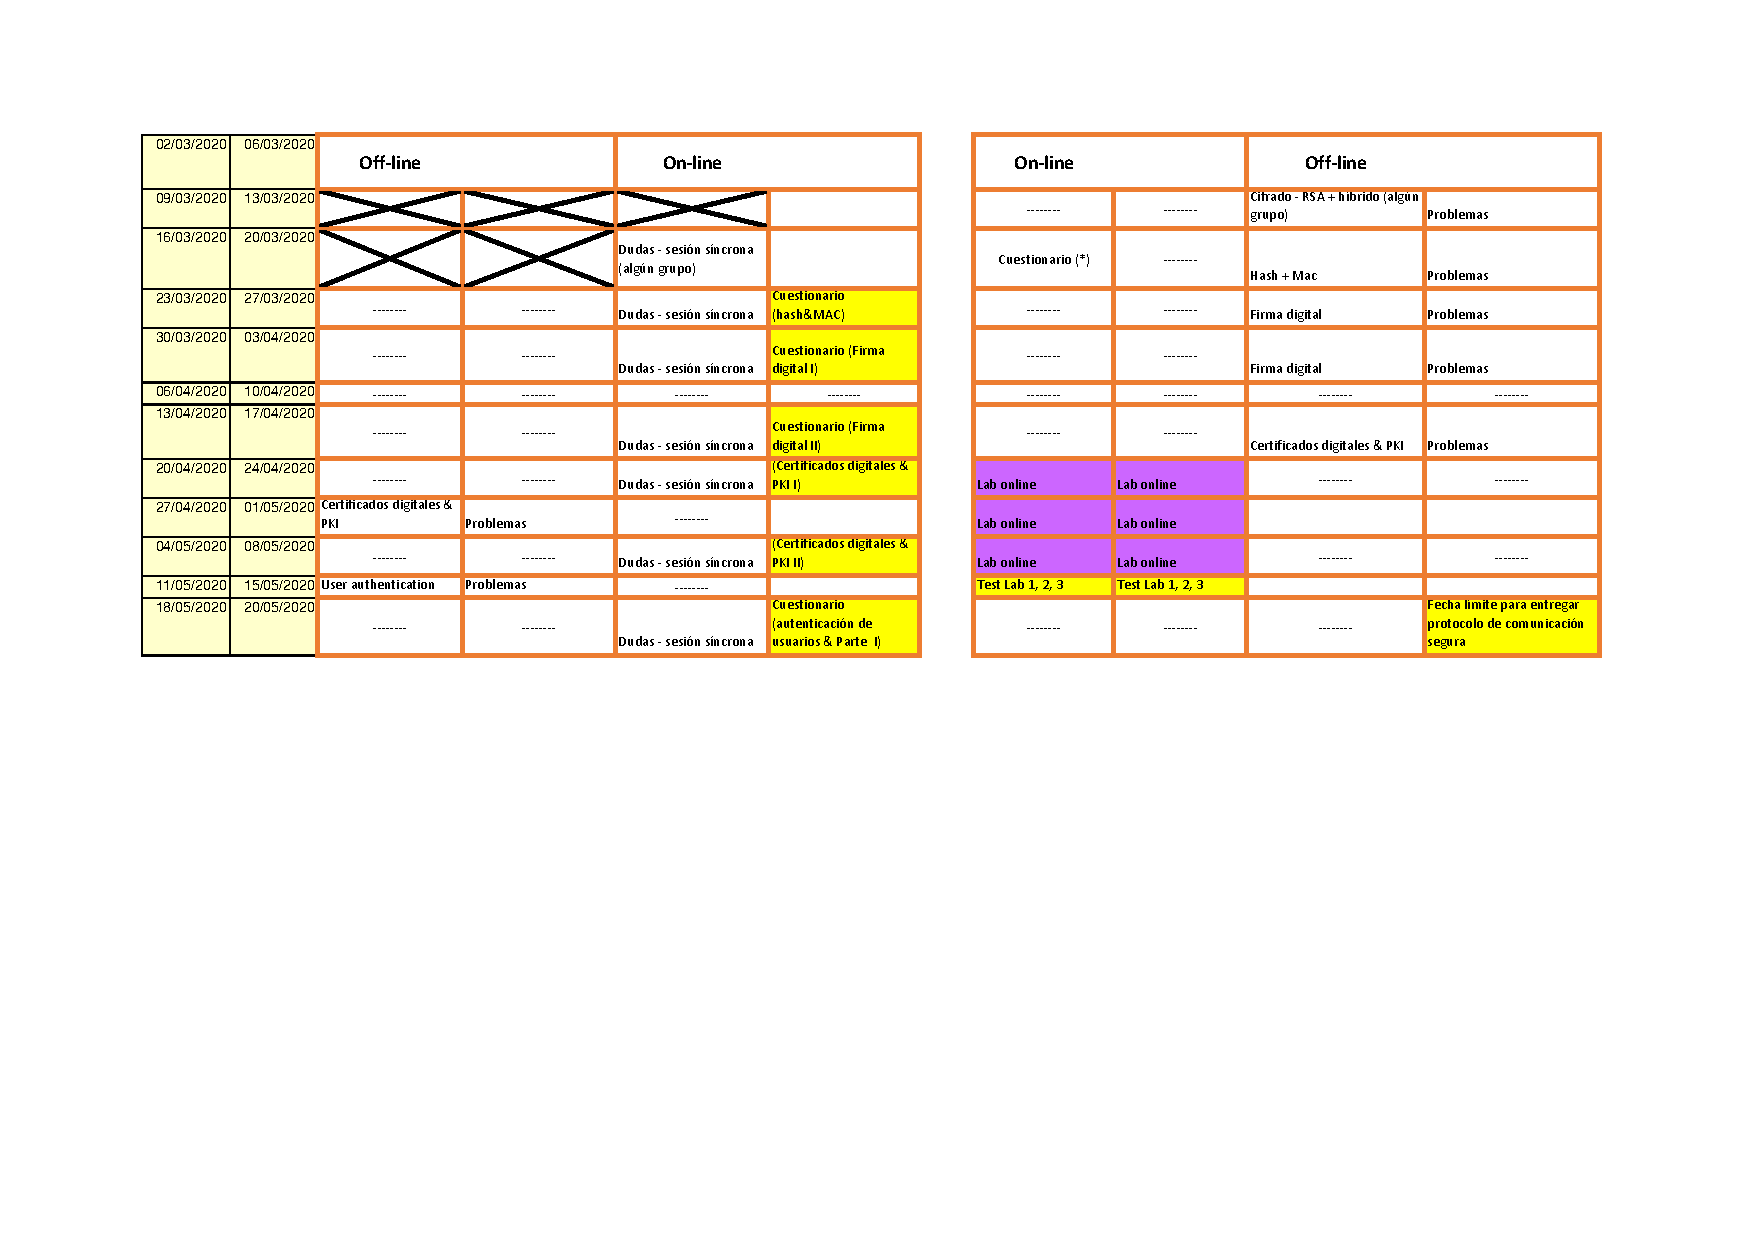
\includepdf[pages=-]{docs/Planificacion_CSI_COVID_ES.pdf}
\includepdf[pages=-]{docs/PlanificacionDocenteCSI1920_version2020.enero.13.ALUMNOS-ES.pdf}
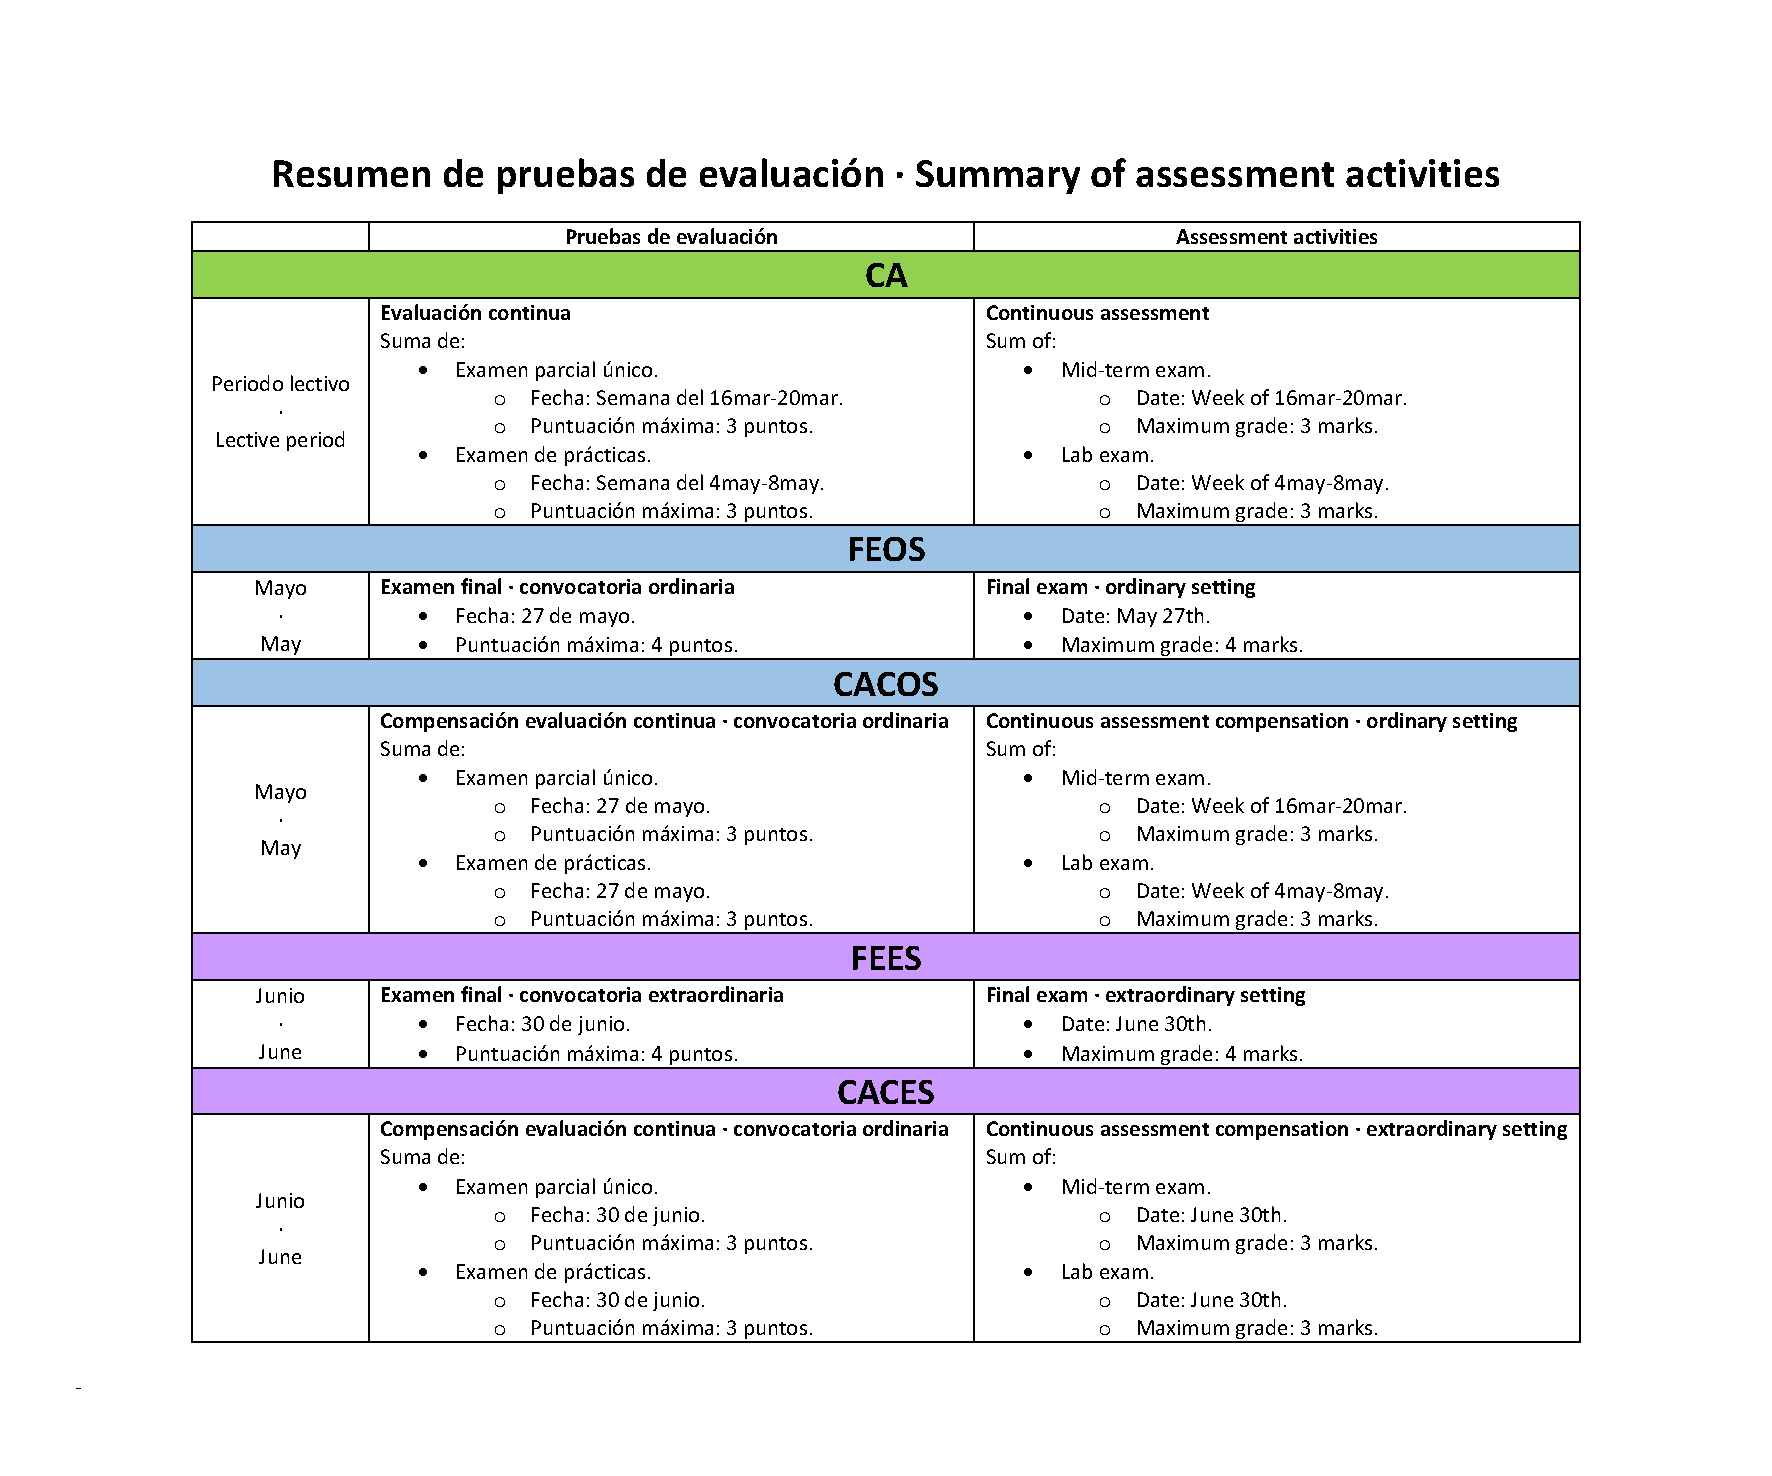
\includepdf[pages=-]{docs/GuiaEvaluacionCSI-1920.pdf}
\includepdf[pages=-]{docs/GuiaAsignatura_1920_14.01.2020_ES.pdf}
\includepdf[pages=-]{docs/Evaluacion_CSI_COVID_ES.pdf}

\part{Resumenes}
\chapter{Tema 1: Fundamentos Matemáticos}

  \textbf{Estructuras}: Sea a, b $\in$ Z, Z tiene estructura de:
  

  \begin{itemize}
  \item \textbf{Grupo (Z, +)} si cumple las siguientes propiedades:
    

    \begin{itemize}
    \item Cierre, a+b sigue perteneciendo a Z
      
    \item Asociativa, a+(b+c) =(a+b)+c
      
    \item Identidad, a+0=0
      
    \item Inverso, a+(-a)= 0
      
    \end{itemize}
  \item \textbf{Grupo Conmutativa o Abeliano} si además de las Grupo cumple:
    

    \begin{itemize}
    \item Conmutativa, a+b=b=a
      
    \end{itemize}
  \item \textbf{Anillo (Z, +, *)} si cumple las de anillo y además para el
    producto:
    

    \begin{itemize}
    \item Cierre
      
    \item Asociativa
      
    \item Identidad
      
    \item * es distributiva respecto +, a*(b+c)= (a*b)+(a*c)
      
    \end{itemize}
  \item \textbf{Anillo Conmutativo} si además de las de Anillo cumple la
    conmutativa.
    
  \item \textbf{Anillo de División} si cumple las de anillo y además:
    Inverso, a*a\^{}1=1
    
  \item \textbf{Cuerpo}: Anillo de División Conmutativo.
    
  \end{itemize}

  
  \textbf{Congruencias:} Sean a, b, n $\in$ Z, a y b serán congruentes
  módulo n ($a \equiv b  \mod n$)
  

  \begin{itemize}
  \item Si la diferencia entre a y b es un múltiplo de n. \textbf{a-b=n*k /
    k entero}
    
  \item También si ambos dejan el mismo resto si los dividimos por n.
    
  \item \textbf{Clase de congruencias de a módulo ([a]):} Conjunto de
    todos los números congruentes con a módulo n, se genera sumando y
    restando n. $[3]_{10}=\{..., -17, -7, 3, 13, 23,...\}$
    
  \end{itemize}

  
  \textbf{Reducción módulo n:} Se busca que a sea un valor entre 0 y
  n-1.
  

  \begin{itemize}
  \item Restar/Sumar n hasta quedarse con el número positivo más bajo.
    

    \begin{itemize}
    \item 16 mod 5=16-15 mod 5=1 mod 5
      
    \end{itemize}
  \item Dividir entre n, y quedarse con el resto. 16 mod 5= 1 mod 5
    
  \end{itemize}

  
  \textbf{Conjunto Z:} Conjunto de clases de congruencia respecto al
  módulo n. Va desde 0 hasta n-1.
  

  \begin{itemize}
  \item
    
	$Z_7 = \{0, 1, 2, 3, 4, 5, 6\}$
    
  \end{itemize}

  \begin{itemize}
  \item \textbf{Operación suma/resta/producto + /- /*} : Siendo los términos
    respecto a mismo módulo, consiste en hacer la operación entre sus
    valores y el resultado módulo n.
    
  \item $[2]+_5[4]=(2+4) \mod 5 = 6 \mod 5 = 1 \mod 5 = [1]$
  \item \textbf{Principios fundamentales de la Aritmética Modular:}
    

    \begin{itemize}
    \item (a + b) (mód. n) = (a(mód. n) + b(mód. n))(mód. n)
      
    \item (a*b) (mód. n) =(a (mód. n) * b (mód. n)) (mód. n)
      
    \item (a*(b+c)) (mód. n) =((a* b) (mód. n)+(a*c) (mód. n)) (mód. n)
      
    \end{itemize}
  \end{itemize}

  
  \textbf{Cálculo de Inversos:} El m.c.d de a y n debe ser 1, para que
  sean \underline{coprimos}(el único divisor que tiene en común es el
  1). \textbf{a\^{}(-1)*a=1. a*x=1 mod n. x=a\^{}(-1) mod n}
  

  \begin{itemize}
  \item \textbf{Teorema de Fermat:} Si \underline{p es primo} y mcd(a, p)=1,
    se cumple:
    

    \begin{itemize}
    \item $a^{p-1} \mod p = 1$ por lo tanto el inverso es $a^{-1} = a^{p-2} \mod p$
      
    \end{itemize}
  \item \textbf{Teorema de Euler:} mcd(a, n)=1, aunque no tiene por qué ser
    primo, se cumple:
    

    \begin{itemize}
    \item $a^{\phi(n)} \mod n = 1$ y para el inverso es $a^{\phi(n)-1} \mod n = a^{-1}$
      
    \item Indicador de Euler: Indicador del numero de elementos de Zn*
    \begin{itemize}
		\item Para p primo $\phi(p)=p-1$, $\phi(p^x)=p^{x-1}(p-1)$, $\phi(p\cdot q) = \phi(p)\cdot\phi(q)$
	\end{itemize}
      
    \item \textbf{Conjunto $Z_n^*$:} Conjunto de números que son coprimos con n.
      

      \begin{itemize}
      \item
        
		$Z_{1 2}^* = \{ 1, 5, 7, 11\} \phi(12) = \phi(2^2\cdot 3)=2^1 \cdot 1 \cdot 2 = 4$
        
      \end{itemize}
    \end{itemize}
  \item \textbf{Algoritmo de Euclides:} Permite hallar el mcd de dos números
    enteros positivos sin necesidad de factorizar los números. También
    permite hallar el inverso de un numero respecto a otro cuando el mcd
    de ambos es 1(coprimos), y despejar el 1.
    

    \begin{itemize}
    \item Ejem: mcd de 1547 y 560, poner el mayor igualado al menor por un
      entero, más resto.
      
    \item 1547 = 2 · 560 + 427
      
    \item 560 = 1 · 427 + 133
      
    \item 427 = 3 · 133 + 28
      
    \item 133 = 4 · 28 + 21
      
    \item 28 = 1 · 21 + 7
      
    \item 21 = 3 · 7 + 0
      
    \item m.c.d.(1547,560) = 7
      
    \item Ejem: cálculo de inverso de 23x mod 25, ir dejando el resto 1
      mediante todas las ecuaciones y el inverso será el que acompaña al
      23.
      
    \item 25=1·23+2
      
    \item 23=11·2+1
      
    \item 11=11·1+0
      
    \item mcd(25, 23)= 1 Coprimos podemos hallar el inverso.
      
    \end{itemize}
  \item \textbf{ax=b mod. n} debe cumplirse mcd(a, n)\textbar b:
    

    \begin{itemize}
    \item Si mcd(a, n)= 1, hay una solución. Se resuelve el inverso de a y
      se multiplica por b.
      
    \item Si mcd(a, n)=m!=1, hay m soluciones. Se simplifica la expresión y
      se resuelve como el anterior, con la diferencia de que las
      soluciones serán con el módulo original y se harán crearan el
      resto de soluciones sumando el módulo del simplificado.
      
    \item Otro método es con Ecuaciones diofánticas: ax+ny=b, simplificamos
      la expresión y damos valor a x e y, y operamos para que quede el
      =b simplificado. Se resta la expresión en la que hemos dado valor
      a x e y con la original simplificada. Dando valor a k, hallamos
      las soluciones x.
      
    \end{itemize}
  \item \textbf{Cuerpos de Galois CG(p):} Sea Zp=\{0, 1, 2,..., p-1\} siendo
    p primo. Zp es un cuerpo finito denominado Cuerpo de Galois CG(p).
    Zp=CG(p)
    

    \begin{itemize}
    \item Zp es un cuerpo respecto a la suma y la multiplicación.
      
    \item Hay p elementos en GC(p).
      
    \end{itemize}
  \item \textbf{Cuerpos de Galois $CG(q^n)$:} Está formado por los
    polinomios de grado n-1 o menor. Si al operar obtenemos un polinomio
    de grado n o mayor, se reduce módulo de un polinomio p(x), que nos
    lo dan y normalmente es: \textbf{p(x)=x\^{}n+x+1} para n= 1, 3, 4,
    6, 7, 9, 15, 22, 28, 30, 46,...
    

    \begin{itemize}
    \item Existen $q^n$ polinomios en $CG(q^n)$. Ejem: CG(2³) 0, x, x², 1,
      x+1, x²+1, x²+x+1, x²+x.
      
    \item Hay q\^{}n -1 elementos coprimos con p(x), la identidad de Euler
      de p(x).
      
    \item Operaciones:
      

      \begin{itemize}
      \item \textbf{Suma y resta:} c(x)=a(x)+-b(x) mod p(x) consiste en
        sumar/restar a y b.
        
      \item \textbf{Multiplicación}: c(x)=a(x)*b(x) mod p(x)
        
      \item \textbf{Dividir(inverso multiplicativo):} u(x)*s(x)=v(x) mod
        p(x)
        

        \begin{itemize}
        \item s(x)\^{}(-1) mod p(x) = s(x)\^{}($\phi$(p(x)) -1) mod p(x) =
          s(x)\^{}(q\^{}n -2) mod p(x)
          
        \end{itemize}
      \end{itemize}
    \end{itemize}
  \item \textbf{Cuerpos de Galois CG(2\^{}n):} Se representa mediante los
    coeficientes 0 y 1. El número de elementos del cuerpo es 2\^{}n. Se
    emplean n bits para representar un elemento.
    

    \begin{itemize}
    \item Ejm: CG(2³) 0 (0 0 0), x (0 1 0), x² (1 0 0), 1 (0 0 1), x+1 (0 1
      1), x²+1 (1 0 1), x²+x+1 (1 1 1), x²+x (1 1 0).
      
    \item Operaciones:
      

      \begin{itemize}
      \item \textbf{Suma y resta}: Consiste en hacer XOR, si son iguales es
        0 y si son distintos 1.
        

        \begin{itemize}
        \item 101+111=010. 110-011=101. Es sumar sin acarreo.
          
        \end{itemize}
      \item \textbf{Multiplicación:} Es la operación lógica AND, es
        multiplicar los números y sumar con XOR. Si se sobre pasa el
        grado de p(x), se reduce a mod p(x) o podemos hacerlo dividiendo
        y cogiendo el resto. 100*100=10000 Habría que dividirlo, ya que
        sobre pasa el grado 3.
        
      \item \textbf{División:} Es hallar el inverso multiplicativo,
        a\^{}(-1)=a\^{}(a\^{}n -2) mod p(x), vamos separando términos y
        operador hasta reducirlo. También se puede hacer dividiendo
        normal, buscando que tenga el mismo grado y restando con XOR.
        
      \item \textbf{xtime:} Es multiplicar por x, que equivale a multiplicar
        por 10. Desplazar 1 a la izq. Se utiliza para simplificar, ya
        que si tiene 0 a la derecha está multiplicado por 10, y de esta
        manera podemos reducirlo a multiplicar 10, x veces.
        

        \begin{itemize}
        \item Es lo utilizado por los computadores. $100^6 = (x^2)^6=x^{12}$. 10 a la
          12
          
        \end{itemize}
      \end{itemize}
    \end{itemize}
  \item \textbf{Restos potenciales:} Son los restos resultado de hacer el
    modulo n de las potencias de un numero a.
    
  \item \textbf{Gaussiano:} Es el menor exponente de la base a que da resto
    1 módulo n, se busca el más bajo por lo que si no se encuentra uno
    por dejo de la identidad de Euler de n, el gaussiano será la
    identidad de Euler y además será generador. Los posibles exponentes
    son divisores de $\phi(n)$.
    
  \item \textbf{Raíces primitivas o generador:} Cuando el gaussiano de un
    número coincide con la identidad de Euler del módulo. Para calcular
    si un número lo es, hay que comprobar las potencias con exponentes
    que sean divisores de la identidad de Euler del módulo, y a la vez
    que esos valores sean menores que la identidad. Exponentes x:
    x\textbar $\phi$(n) y x\textless $\phi$(n)
    
  \item \textbf{Logaritmos discretos:} Calculó inverso a la exponenciación
    en la aritmética modular. Para hallar b, buscamos en los restos
    potenciales de a el valor b, y la columna que contenga el b será la
    x.
    

    \begin{itemize}
    \item
      
	  $a^x = b \mod n x=\log_a(b) \mod n$
      
    \end{itemize}
  \end{itemize}

  
\chapter{Tema 2: Introducción a la Criptografía.}

  Se hace uso de una clave y un algoritmo de cifrado. Si la misma clave
  sirve para cifrar y descifrar es un cifrado simétrico.
  
  \textbf{Criptografía:} Disciplina que estudia los principios, métodos
  y medio de transformar los datos para ocultar su significado,
  garantizando su integridad(que no hayan sido modificados), su
  autenticidad(asegurarnos quien ha sido el autor) y prevenir su
  repudio(que no se pueda negar la autoría.
  

  \begin{itemize}
  \item Elementos básicos:
    
    \begin{itemize}
    \item \textbf{Espacio de mensajes:} Mensajes en claro, que no han sigo
      transformados. M=\{m1,m2,...\}
      
    \item \textbf{Espacio de cifrados:} Mensajes que ya han sido
      transformados. C=\{c1,c2,...\}.
      
    \item \textbf{Espacio de claves}: Sirve para configurar el algoritmo de
      cifrado/descifrado. K=\{k1,k1,\ldots\}
      
    \end{itemize}
  \item Las transformaciones pueden ser:
        \begin{itemize}
    \item \textbf{Cifrado M-\textgreater C:} Entra un mensaje en claro,
      mediante un cifrador y una clave, pasa a ser un mensaje cifrado.
      
    \item \textbf{Descifrado C-\textgreater M}: Proceso inverso al cifrado,
      pasa de cifrado a en claro.
      
    \end{itemize}
  \item Características de los sistemas criptográficos:
        \begin{itemize}
    \item Tipo de operaciones realizadas: Generalmente, sustitución y
      transposición, no puede perderse información.
      
    \item \textbf{Numero de claves usadas:}
      
      \begin{itemize}
      \item \textbf{Simétricos}: Hay una sola clave, tanto para cifrar como
        para descifrar.
        
      \item \textbf{Asimétricos}: Se cifra con una clave pública, que es
        conocida, y se descifra con una clave privada, no conocida.
        
      \end{itemize}
    \item \textbf{Tipo de procesamiento del texto en claro:}
      
      \begin{itemize}
      \item \textbf{Por bloques}: Va cifrando trozos de cadena.
        
      \item \textbf{Flujo continuo:} Se hace sobre pequeños trozos como
        bytes o bits.
        
      \end{itemize}
    \end{itemize}
	\pagebreak
  \item Codificador vs. Cifrador:
    
    \begin{itemize}
    \item \textbf{Codificador}: Se sigue una función conocida, que siempre
      es igual. Morse, ASCII,\ldots{}
      
    \item \textbf{Cifrador}: Se sigue un proceso que no es conocido por
      todos y que varía, y es necesaria una clave.
      
    \end{itemize}
  \end{itemize}

  
  \textbf{Criptoanálisis}: Ciencia que trata de frustrar las técnicas
  criptográficas, trata de obtener la clave de cifrado y si no es
  posible al menos descifrar el mensaje.
  

  \begin{itemize}
  \item \textbf{Principio de Kerchoff:} La seguridad del cifrado debe
    residir en el secreto de la clave.
    
  \item No debe ser por falta de claridad que es segura.
    
  \item Los ataques se basan en el conocimiento sobre el algoritmo y en
    posible información adicional.
    
  \item Métodos:
    
    \begin{itemize}
    \item \textbf{Ataques al algoritmo:} Se basa en el conocimiento del
      algoritmo, y desarrolla métodos en función de como funciona.
      Además del algoritmo el atacante puede conocer el texto descifrado
      de otro dado cifrado con la misma clave, textos escogidos por el
      atacante pero cifrados. Conoce algoritmo y/o algún ejemplo de
      texto descifrado con su correspondiente cifrado. Cuanta menos
      información más difícil será de resolver.
      
    \item \textbf{Fuerza bruta:} Consiste en probar todas las claves
      posibles, en media se probarán la mitad de las posibilidades para
      tener éxito. Este proceso requiere tiempo y aumenta
      exponencialmente al aumentar el tamaño de la clave. Lo primero que
      se prueban son combinaciones de palabra del diccionario, cuando
      esto tenga sentido.
      
    \end{itemize}
  \item \textbf{Algoritmo de cifrado incondicionalmente seguro:} No se
    filtra información por muy largo que sea el texto cifrado. Solo lo
    cumple el cifrador Vernam, y en ciertas condiciones(clave realmente
    aleatoria, usarla una sola vez y de longitud igual o superior al
    texto a cifrar). Pero no es práctico, es muy difícil conseguir
    claves con esa condición.
    
  \item \textbf{Algoritmo de cifrado matemáticamente vulnerable:} Al
    aumentar la longitud del texto cifrado se filtra información, es lo
    que le ocurre al resto de algoritmos que no son Vernam.
    
  \item \textbf{Seguridad computacional:} Se requiere tantas operaciones que
    el tiempo en realizarlas es mayor que el tiempo útil de la
    información. Por lo que para cuando se ha resuelto no es útil ya.
    También puede ser que el coste de resolverlo sea superior al de la
    propia información.
    
  \item \textbf{Los cifradores simétricos} solo se pueden resolver mediante
    un ataque de fuerza bruta, no existe un algoritmo.
    
  \end{itemize}

  
  \textbf{Teoría de la información:} Establece una medida para evaluar
  el secreto de un cifrador, que se basa en la incertidumbre que tiene
  el criptoanalista sobre el texto en claro al interpretar su cifrado.
  

  \begin{itemize}
  \item Sean m1, m2,\ldots{} mensajes independientes con probabilidad de
    ocurrencia (de que se repita) p(m1), p(m2),\ldots{}
    
  \item La \textbf{cantidad de información (ci)} de un mensaje mi es: $C_i=-\log_2 p(m_i)$ bits. Un
    mensaje que se repite, alta probabilidad de ocurrencia aporta menos
    información que un mensaje único. Mayor p(mi), menor ci
    
  \item \textbf{Entropía}: Es el promedio de información transportada por un
    mensaje. Y la previsible tras la aparición de un mi. Mayor entropía,
    mayor incertidumbre.
    
    \begin{itemize}
    \item Sea la fuente de mensajes M: $H(M)=-\Sigma_i p(m_i) \log_2 p(m_i)$ bits
      
    \item H(M)=0 cuando p(mi)=1, ya que no aporta información si siempre
      aparece.
      
    \item H(M)=máxima=log2 n cuando p(mi)=1/n.
      
    \end{itemize}
  \item \textbf{Entropía condicionada:} Cuando existe alguna relación entre
    las apariciones de dos mensajes consecutivos de distinta fuente, la
    presencia del primero disminuye la incertidumbre del segundo.
    Conocer el primero me facilita encontrar el segundo. Los métodos
    tratan de maximizar H(M\textbar N) para poder relacionar el conjunto
    de textos claros M y el de textos cifrados N.
 
    \begin{itemize}
    \item $H(M/N) =-\Sigma_j p(n_j)\cdot \Sigma_i p(m_i/n_j) \log_2 p(m_i, n_j)$
      
    \end{itemize}
  \end{itemize}

  
  \textbf{Aleatoriedad:} Sea S un espacio muestral con distribución de
  probabilidad P, cada posible valor que X puede tomar en S tiene
  asociada una determinada probabilidad.
  

  \begin{itemize}
  \item \textbf{Usos}:
    

    \begin{itemize}
    \item Distribución de claves.
      
    \item Generación de claves de sesión y claves para RSA.
      
    \item Generación de flujos de bits para algoritmos de cifrado simétrico
      de flujo.
      
    \end{itemize}
  \item \textbf{Criterios}:
    

    \begin{itemize}
    \item \textbf{Distribución uniforme}: La frecuencia de aparición de cada
      símbolo debe ser aproximadamente la misma(tantos 0's como 1's)
      
    \item \textbf{Independencia}: Ninguna su secuencia puede ser inferida de
      otra.
      
    \end{itemize}
  \item Se pueden hacer pruebas que comprueben que se cumple la uniformidad,
    pero no hay pruebas que comprueben la independencia, pero sí que no
    es independiente.
    
  \item \textbf{Pseudoaleatoriedad(PRNG):} Pasan las pruebas de
    aleatoriedad, pero tienen un mecanismo determinista, algoritmo, que
    genera los números. Aunque un algoritmo no es verdaderamente
    aleatorio.
    
  \item \textbf{Aleatoriedad(TRNG):} Mecanismo no determinista, ciertos
    procesos naturales y eliminación del sesgo con funciones resumen.
    
  \end{itemize}

  
  \textbf{Complejidad algorítmica:} Estudia los algoritmos bajo la
  dificultad de su resolución. Clasifica los algoritmos según su
  complejidad. Turing demostró que no todos los problemas tiene un
  algoritmo que lo resuelva.
  

  \begin{itemize}
  \item \textbf{Clasificación}:
    

    \begin{itemize}
    \item \textbf{Indecidible}: No hay algoritmo que lo resuelva.
      
    \item \textbf{Decidible}: Existe al menos un algoritmo que lo resuelve.
      
    \item \textbf{Intratable}: No se puede resolver en un tiempo razonable.
      
    \item \textbf{Tratable}: Resuelve cualquier problema particular en un
      tiempo razonable.
      
    \end{itemize}
  \item La complejidad se mide en \textbf{tiempo (t)} según el tamaño de la
    \textbf{entrada (n)}. Puede ser:
    

    \begin{itemize}
    \item \textbf{Polinómica}: El tiempo es de orden polinómico o menor.
      

      \begin{itemize}
      \item \textbf{Lineal}: $O(n)$
        
      \item \textbf{Logarítmico}: $O(\log n)$
        
      \item \textbf{Polinómico}: $O(n^c)$
        
      \end{itemize}
    \item \textbf{Exponencial}: El tiempo t es de orden mayor que polinomio.
      

      \begin{itemize}
      \item \textbf{Exponencial}: O(c\^{}x)
        
      \item \textbf{Factorial}: O(n!)
        
      \end{itemize}
    \end{itemize}
  \item Los problemas se clasifican en:
    

    \begin{itemize}
    \item \textbf{Clase P}: Problemas decidibles, tratables, algoritmo
      determinista(cada paso se resuelve de manera única, una opción
      solo) y polinómico (buenos algoritmos).
      
    \item \textbf{Clase NP}: Problemas tratables e intratables, algoritmo no
      polinómico (malos) y no determinista, en cada paso hay que seleccionar una opción.
      
    \end{itemize}
  \end{itemize}

  \pagebreak
  \textbf{2.2 Métodos Criptográficos clásicos:}
  

  \begin{itemize}
  \item \textbf{Transposición}: Consiste en alterar el orden de los
    caracteres, pero sin modificarlos.
    

    \begin{itemize}
    \item \textbf{De riel}: Se hacen 2 columnas, un carácter va una columna
      y el siguiente a la otra. Después se concatenan las dos columnas,
      la segunda se añade al final de la primera.
      
    \item \textbf{Por grupos, permutación}: Consiste en ir alterando el
      orden de los caracteres en grupos de caracteres. Se divide la
      cadena en grupos y se lleva a cabo el proceso. Indicando en que
      posición irá cada uno.
      
    \item \textbf{Por series}: Ordenar mensajes como cadena de submensajes.
      Se hacen funciones o series que se concatenan y cada una coge
      ciertos caracteres (primos y no primos), y las suma de todas
      recoge todos los caracteres.
      
    \item \textbf{Por columnas/filas}: Introducir la cadena original en una
      estructura o patrón, e ir alterando el orden de las filas o
      columnas. La cadena codificada será la originada de ese desorden
      de la estructura.
      
    \end{itemize}
  \item \textbf{Sustitución}: Consiste en intercambiar los caracteres de la
    cadena original por otros de un alfabeto codificado.
    

    \begin{itemize}
    \item \textbf{Monoalfabeto} \textbf{monográfica}(\textbf{simple)}: Ir
      sustituyendo cada carácter por su equivalente cifrado. El
      equivalente consiste en el número de la letra multiplicada por un
      valor, sumándole otro y todo eso módulo del numero de letras del
      alfabeto. Se usa el módulo de ese valor para conocer que letra
      corresponde en la codificación. E(m)=(am+b) mod n, la a es la
      constante de decimación, la b la constante de desplazamiento (a y
      b forman la clave y deben ser coprimos) y n el número de letras
      del alfabeto. Para descifrar consiste en invertir el proceso, se
      despeja la expresión modular. E(m)=7m+3 mod 27=n
      D(n)=(n-3)7\^{}(-1) mod 27
      

      \begin{itemize}
      \item \underline{Cifrador por desplazamiento puro}, E(m)=(m+b) mod n
        

        \begin{itemize}
        \item Cifrador Cesar, E(m)=(m+3) mod n
          
        \end{itemize}
      \item \underline{Cifrador por decimación pura}, E(m)=(am) mod n
        
      \item \underline{Cifrador por sustitución afín}, E(m)=(am+b) mod n
        
      \end{itemize}
    \item \textbf{Monoalfabeto poligráfica}: Sustitución n (n\textgreater=2)
      caracteres texto-claro por n caracteres texto-cifrado.
      

      \begin{itemize}
      \item \textbf{Playfair}: Se hace una matriz que comienza con las
        letras de una clave, sin que se repitan letras y el resto de la
        matriz se rellena con el resto de las letras en orden. Para
        todas las letras se usa una matriz 5x5, algunas como la
        \textbf{\underline{ñ y j}} están en casilla con otra. Se separa
        la cadena en grupos de caracteres (2) y se consulta la posición
        de las letras en la matriz y según unos criterios(derecha y
        abajo, si están en la misma fila, se coge la inmediata a la
        derecha de cada una, si están en la misma columna es el
        inmediato de abajo, y si están en diagonal se hace espejo,
        perpendicular a la flecha que los conecta) se eligen como
        caracteres codificados unos desplazados en la matriz. Para
        descodificar se necesita la misma matriz, la cadena codificada y
        los criterios se hacen a la inversa, izquierda y arriba.
        
      \item \textbf{Hill:} Dividimos la cadena en vectores de tamaño n, es
        capaz de cifrar ``n''caracteres a un tiempo. La clave es una
        matriz nxn que multiplicaremos por los vectores formados por los
        grupos de la cadena, lo realizamos para toda la cadena y la
        cadena cifrada es el resultado de concatenar todos. Para
        descifrar hallamos el inverso de la matriz(
        ($adj(nxn)^{det(nxn)}$) y lo multiplicamos por los vectores
        cifrados. Los valores deben estar en mod numero de letras.
        
      \end{itemize}
    \item \textbf{Polialfabeto periódica: Vigenére}
      

      \begin{itemize}
      \item Hay 27 alfabetos, uno para cada letra, que comienza desde esa
        letra. Ejem: Alfabeto de C E(mj) = (mj+k\^{}sub(j mód m)) mód.
        27
        
      \item \textbf{Con clave:} Lo que equivale a colocar bajo la cadena
        original la clave tantas veces como para cubrirla entera. Y lo
        que se hace es buscar en el alfabeto de la letra de la
        clave(fila) la posición de la letra de la cadena original(parte
        alta de la tabla). Para descifrar colocamos también la clave
        bajo la cadena codificada y mirando la fila de la letra de la
        clave buscamos dentro de la misma la letra de la cadena
        codificada y la letra correspondiente en la cabecera será el
        carácter descodificado.
        
      \item \textbf{Con autoclave:} Consiste en colocar una vez la clave
        bajo la cadena original y a continuación la cadena a codificar
        también como clave, hasta que cada letra de la cadena original
        le corresponda uno de clave. Para codificar se miran la fila de
        la letra de la clave y buscamos en la cabecera de las columnas
        el carácter que le corresponde de la original, así hasta
        completar la cadena. Para descodificar colocamos la clave una
        vez, y comenzamos a descodificar los caracteres de la cadena
        codificada que tienen otro de la clave, para ello mirando la
        fila de la clave buscamos dentro de la fila la letra codificada
        y el valor que le corresponda en la cabecera será el
        descodificado, y cuando necesitamos más caracteres de clave
        vamos poniendo la cadena descodificada.
        
      \end{itemize}
    \item \textbf{Polialfabeto no periódica: Vernam}
      

      \begin{itemize}
      \item La longitud de la clave es igual o mayor que la longitud del
        texto sin codificar, los valores son aleatorios, lo que la hace
        perfecta. Los problemas son el tamaño de la clave y que no se
        puede reutilizar. XOR del valor de cada letra de la cadena con
        su correspondiente en la clave, y si el valor supera el número
        posible de caracteres, hacemos mod numCaracteres.
        
      \item Para codificar: ci= E(mi) = (mi XOR ki)
        
      \item Para descodificar: mi= E(ci) = (ci XOR ki)
        
      \end{itemize}
    \item \textbf{Máquina Enigma:}
      

      \begin{itemize}
      \item Cifrado/descifrado rotatorio.
        
      \item Funciona con rotores que leen una placa en la que están creadas
        las conexiones entre letras...
        
      \end{itemize}
    \end{itemize}
  \item \textbf{Criptoanálisis de Criptografía clásica:}
    

    \begin{itemize}
    \item \textbf{Romper el Cifrado de Desplazamiento:} Consiste en fuerza
      bruta, ir probando todos los posibles valores de la constante de
      desplazamiento(n) que pueden ir desde 0 hasta el
      tamañoAlfabeto-1(ya que si supera ese tamaño al hacer mod equivale
      a uno menor)
      

      \begin{itemize}
      \item Codificar: E(x)=(x+n) mod m. Descodificar: D(x)=(x-n) mod m
        
      \end{itemize}
    \item \textbf{Romper el Cifrado de Sustitución Monoalfabeto:} Para no
      hacerlo por pura fuerza bruta, se analiza la frecuencia de
      aparición de ciertos caracteres y vamos relacionándolos con los
      caracteres más frecuentes de nuestro alfabeto, ya que la
      frecuencia se transmite al codificar. Suponiendo dos parejas en
      los que uno de los más frecuentes codificado es otro de los más
      frecuentes propios del alfabeto, creamos un sistema de ecuaciones
      con sus valores y buscamos resolverlo y probar si tienen sentido
      ese resultado. Y mediante la prueba y error de los más frecuentes
      hallaremos los valores de las constantes.
      

      \begin{itemize}
      \item E(m)=(am+b) mod n
        
      \item Algunas técnicas para dificultarlo son: Cadenas suficientemente
        cortas, evitar emplear las letras más frecuentes o evitar
        terminaciones que se repiten con frecuencia en las palabras.
        
      \end{itemize}
    \item \textbf{Romper el Cifrado de Sustitución Polialfabeto:}
      \underline{Método de Kasiski} e \underline{Índice de
      Coincidencia.} Consiste en ir calculando el IC de subcadenas de la
      cifrada, estas subcadenas se originan de ir saltándose x letras,
      pero crear tantas cadenas como se pueda con ese tipo de salto.
      Aquellas subcadenas que tengan un IC similar al de un lenguaje
      indicaran el tamaño de la clave de Vigenére. Conociendo el tamaño
      de la clave aplicamos Asistí (este obtendría el tamaño de la
      clave observa ando repeticiones en la cadena y midiendo su
      separación y el tamaño sería el mcd de esas separaciones), que
      consiste en dividir la cadena en tantos grupos como tamaño tiene
      la clave, así tenemos agrupadas aquellas letras que perteneces al
      mismo alfabeto. Dentro de esos grupos observamos la frecuencia de
      aparición de cada carácter y haremos combinaciones cogiendo un
      carácter de cada grupo y probaremos si esa es la clave, lo hacemos
      descifrando normal mirando la fila de la letra de la clave y
      dentro de ella el carácter codificado.
      
    \end{itemize}
	\pagebreak
  \item \textbf{Índice de Coincidencia:} Medida estadística sobre un texto.
    Es la probabilidad de que dos letras seleccionadas aleatoriamente en
    un texto sean la misma.
    

    \begin{itemize}
    \item Se calcula con: $\frac{\Sigma(f_i \cdot (f_i - l))}{N(N-l)}$
      
    \end{itemize}
  \end{itemize}

  
  \textbf{2.3 Criptosistemas simétricos:} El mensaje se descompone en
  bloques de símbolos de igual longitud, y todos los bloques se cifran
  con la misma clave, y el proceso inverso descifra.
  

  \begin{itemize}
  \item Clasificación:
    

    \begin{itemize}
    \item \textbf{Tipo de operaciones realizadas:} En general, sustitución y
      permutación. No puede perderse información.
      
    \item \textbf{Número de claves usadas}:
      

      \begin{itemize}
      \item \textbf{Simétricos}: Con una clave, que es secreta y sirve para
        cifrar y descifrar.
        
      \item \textbf{Asimétrico}: Con dos claves, una pública para cifrar que
        es conocida y otra secreta que no es conocida para descifrar.
        Para transmitir la clave privada se cifra simétricamente, cuando
        se ha descifrado la simétrica ya tenemos la clave secreta para
        descifrar el mensaje público.
        
      \end{itemize}
    \item \textbf{Tipo de procesamiento:} Por bloques o Flujo continuo.
      
    \end{itemize}
  \item \textbf{Esquema de Feistel:} Es un cifrador de bloque, con $2^n$!
    posibles claves, siendo n el tamaño del bloque de texto y k el
    tamaño de la clave, k\textless=n. Hay alta difusión, cada valor de
    la cadena cifrada depende de muchos de la cadena original, se
    consigue permutando, cifrado y permutando de nuevo y una alta
    confusión, busca complicar la relación estadística entre C y k, se
    logra con sustituciones complejas.
    

    \begin{itemize}
    \item La cadena tras la transformación inicial, se parte en dos, la
      parte derecha pasa a ser la parte izquierda. La parte izquierda
      tras hacer un XOR con la parte derecha tras pasar por una función
      de ronda F, se pone como parte derecha. Y este proceso se repite
      una serie de veces, para dar más seguridad. Se cifra y descifra de
      la misma manera, pero cambiando el orden de las subclaves de la
      función de ronda. Lo más importante de este método es un buen
      método de expansión de claves y una buena función de ronda.
      
    \item Tamaño bloque 64, clave 128, numero de rondas 16. Cuanto mayor sea
      el tamaño más seguridad, pero también será más lento
      
    \end{itemize}
  \item \textbf{Modos de operación:} Técnicas para mejorar el efecto de un
    algoritmo criptográfico, se puede aplicar para cualquier cifrador de
    bloque.
    

    \begin{itemize}
    \item \textbf{Electric CodeBook (ECB):} El mismo bloque a la entrada
      genera el mismo bloque a la salida. Consiste en que cada bloque
      del texto en claro pase por el cifrador de bloque, de esta manera
      obtenemos el bloque cifrado.
      
    \end{itemize}
  \end{itemize}

  


  \textbf{Ventajas}: El cifrado y descifrado se puede hacer en paralelo,
  los errores no se propagan y transmisión segura de un bloque.

  \textbf{Desventajas}: Los bloques repetidos dan como resultado
  criptogramas repetidos, es posible alterar el
  orden/modificar/repetir/eliminar los bloques y necesita relleno el
  ultimo bloque, este indica cierta información sobre el mensaje.

  \begin{itemize}
  \item \textbf{Cypher Block Chaining(CBC):} Se realiza en cadena, cada
    cifrador de bloque recibe el texto claro XOR vector, y da como
    salida el bloque cifrado, que también será el vector del siguiente
    bloque. El primer vector es dado, el IV.
    

    \begin{itemize}
    \item Bloque cifrado=Cifrar con clave K(Bloque en claro XOR Vector)
      
    \item Bloque descifrado= Descifrar(Bloque cifrado m) XOR Bloque cifrado
      m-1
      
    \item Requiere relleno y un error se propaga en dos bloques.
      
    \end{itemize}
  \item \textbf{Cypher FeedBack(CFB):} Usa un registro de desplazamiento y
    opera sobre segmentos más pequeño que el bloque, por lo que se puede
    pasar de cifrado en bloque a flujo. Un error en el cifrado se
    propaga dos bloques.
    
  \end{itemize}

  El vector(texto cifrado anterior o inicial) pasa por el cifrador de
  bloque, de su resultado se escogen los n primeros bits y se hace un
  XOR con el bloque de texto en claro de tamaño n, eso da lugar a ese
  bloque cifrado y al vector del siguiente bloque que desplazará hacia
  la izquierda para hacer el hueco.

  \begin{itemize}
  \item \textbf{Outer FeedBack(OFB):} El vector inicial es un nonce(valor
    aleatorio no utilizado antes), un error en el cifrado afecta a un
    solo bloque y se descartan los bits sobrantes para el último bloque.
    Se puede pasar de cifrado en bloque a uno de flujo.
    

    \begin{itemize}
    \item El vector(el primero el inicial y después el vector anterior
      cifrado), se pasa por el bloque de cifrado y se bifurca, por un
      lado será el vector del siguiente bloque, y por el otro se hace
      XOR con el texto en claro y es el bloque cifrado.
      
    \end{itemize}
  \item \textbf{Counter(CTR):} Utiliza un contador del tamaño de bloque(n),
    se inicializa con un nonce y se le suma 1 mod 2\^{}n en cada bloque,
    se descartan los bits sobrantes. Se puede pasar de cifrado en bloque
    a uno de flujo. Es muy usado por su simplicidad.
    
  \end{itemize}

  El nonce + contador se pasan por el cifrador de bloque, la salida XOR
  bloque en claro da lugar al bloque cifrado.
\pagebreak
  \begin{itemize}
  \item \textbf{Cifradores de bloque: Ventajas y desventajas:}
    

    \begin{itemize}
    \item \textbf{Ventajas:} Alta difusión y confusión en el criptograma, y
      fácil implementación. Son simétricos, el cifrado y descifrado son
      casi idénticos, y son eficientes, muy rápidos.
      
    \item \textbf{Desventajas}: El canal para distribuir las claves, el gran
      numero de claves y que un error se propaga a otros bloques.
      Vulnerable a ataques si se repiten bloques.
      
    \end{itemize}
  \item \textbf{Data Encryption Standard (DES):} Clave de 64 bits, bloques
    de 64 y se hacen 16 rondas.
    

    \begin{itemize}
    \item Se hace una permutación inicial, se hacen 16 rondas y por último
      la permutación final.
      

      \begin{itemize}
      \item Los bloques de texto en claro se presentan como matriz de 8x8
        números escritos por filas.
        
      \item La \textbf{permutación inicial} separa los que ocupan posiciones
        pares de los que ocupan una impar, en dos bloques, y se escriben
        de derecha a izquierda y de arriba a abajo. El bloque de los
        pares es el bloque izquierdo y el otro el derecho.
        
      \item En cada \textbf{ronda} se hace, el bloque derecho pasa a ser el
        bloque izquierdo, pero el bloque izquierdo se hace XOR con el
        resultado de que el bloque derecho recorra: Caja de Expansión,
        XOR con una clave, Caja de Sustitución y Caja de permutación. El
        proceso se repite 16 veces,
        

        \begin{itemize}
        \item \textbf{Caja de expansión}, el bloque pasa de 32 a 48 bits, se
          añade uno a cada lado de las filas de 4 bits. El de la derecha
          es el último de la fila anterior, y el de la izquierda es el
          primero de la siguiente fila.
          
        \item \textbf{XOR} con una clave de 48 bits.
          
        \item \textbf{Caja de Sustitución}, pasa de 48 a 32 bits, cada fila
          se pasa por su propia tabla(hay 8 tablas diferentes), el
          primer y último bit indican la fila en la tabla, y el resto
          indica la columna de la tabla. El valor que corresponda se
          escribe con 4 bits sustituyendo al anterior que ocupa 6 bits.
          
        \item \textbf{Caja de Permutación}, según una tabla cambiamos las
          posiciones de los elementos del bloque.
          
        \item Se hace \textbf{XOR con el bloque izquierdo} y pasa a ser el
          bloque derecho.
          
        \end{itemize}
      \item El \textbf{generado de claves del segundo paso}, genera 16
        claves, una para cada ronda:
        

        \begin{itemize}
        \item Se parte de una clave de 64 bits de la que se quitan 8.
          
        \item Con los 56 bits hacemos una permutación y los dividimos en dos
          bloques de 28 bits. Arriba izq. y abajo derecha
          
        \item Cada bloque de 28 bits se desplaza 1 o 2 posiciones a la
          izquierda, según el ciclo en el que se esté. Para hallar la
          propia solución se juntarán, pero para hallar una de las
          siguientes claves seguimos haciendo desplazamientos.
          
        \item Se juntan ambos bloques según un el orden determinado por la
          tabla.
          
        \end{itemize}
      \item Para descifrar se sigue el proceso inverso, y las claves también
        en orden inverso, en vez de desplazamiento a la izquierda es a
        la derecha.
        
      \item \textbf{Cifrado múltiple}, para DES sí tiene sentido realizar
        cifrado múltiple, el sistema no s un grupo. Por los un aumenta
        la seguridad.
        

        \begin{itemize}
        \item \textbf{3 DES con 2 claves}: La primera vez con la clave 1, el
          segundo con la segunda y el tercero de nuevo con la primera.
          Este es suficiente seguro.
          
        \item \textbf{3 DES con 3 claves}: Una clave para cada ciclo de
          cifrado, apenas se usa, ya que con 2 claves es suficiente.
          
        \end{itemize}
      \item \textbf{Ataques al DES:}
        

        \begin{itemize}
        \item \textbf{Por fuerza bruta}: se puede romper en menos de un día
          con el HW adecuado.
          
        \item \textbf{Con criptografía diferencial}, se necesitan $2^{49}$ textos
          en claro escogidos y sus correspondientes cifrados.
          
        \item \textbf{Con criptografía lineal}, se necesitan $2^{49}$ textos en
          claro conocidos y sus correspondientes cifrados.
          
        \end{itemize}
      \item \textbf{Ataques al Triple DES:} ``Meet-in-the-middle''(meterse
        en el proceso y alterar las claves desde dentro) y los ataque
        con textos conocidos y escogidos.
        
      \end{itemize}
    \end{itemize}
  \item \textbf{Advanced Encryption Standart (AES):} Se utiliza para
    comunicaciones gubernamentales, transferencia de fondos bancarios y
    comunícanos civiles.
    

    \begin{itemize}
    \item Criptografía simétrica, es un cifrador de bloques de 16 bytes.
      
    \item Hay tres longitudes de clave: 128, 192 y 256 bits.
      
    \item Red de sustitución-permutación, pero no es esquema de Feistel, el
      bloque no se divide.
      
    \item Es rápido tanto en software como en hardware, se basa en 4
      funciones invertibles, que para descifrar se hacen su inverso.
      

      \begin{itemize}
      \item El bloque de texto y la clave están compuestos por 16 bytes, que
        se colocan de arriba a abajo y de izquierda a derecha.
        
      \item \textbf{Proceso de cifrado:}
        

        \begin{itemize}
        \item \textbf{Ronda inicial:} AddRoundKey.
          
        \item \textbf{Ronda:} ByteSub, ShiftRow, Mixcolumns y AddRoundKey.
          Se repite este paso.
          
        \item \textbf{Ronda final:} ByteSub, ShiftRow y AddRoundKey.
          
        \end{itemize}
      \item \textbf{Proceso de descifrado:} Se recorre el esquema de abajo
        de arriba, haciendo las funciones inversas.
        
      \end{itemize}
    \item Como la unidad es el byte, se opera en Cuerpos de Galois $GF(2^8)$
      para la suma y multiplicaciones. Para la reducción se hace con el
      polinomio $p(x)=x^8+x^4+x^3+x+1$.
      
    \item \textbf{Las transformaciones:}
      

      \begin{itemize}
      \item \textbf{ByteSub}(sustitución de un byte):
        

        \begin{itemize}
        \item Consiste en hallar el inverso de cada byte y multiplicarlo por
          una matriz fija y el $63_{16}$ (representados como 1's y 0's). Las
          sumas y multiplicaciones sobre el cuerpo de Galois.
          
        \item Otro método es consultar una tabla en la que ya se ha
          realizado el proceso y coger el correspondiente, los primeros
          4 bits fila y los otros 4 columnas, o en hexadecimal. Ej. 5a
          
        \end{itemize}
      \item \textbf{ShiftRow}(desplazamiento de filas): Desplazar bloques de
        un byte hacia la izquierda modulo columna, comenzado por 0 cada
        vez fila desplaza uno más.
        

        \begin{itemize}
        \item Primera fila 0, la segunda 1, la tercera 2 y la cuarta
          desplaza 3 bytes.
          
        \end{itemize}
      \item \textbf{MixColumn}(mezcla de datos dentro de cada columna):
        Opera sobre columnas, que se consideran como polinomios de
        $GF(2^a)$, se multiplica cada columna con una matriz fija de
        números en hexadecimal. Se ponen todos en binario y se opera en
        Galois, teniendo como modulo la $p(x)=x^8+x^4+x^3+x+1$. Se hace para
        todas las columnas.
        
      \item \textbf{AddRoundKey}(añade un clave de vuelta al estado): Se
        hace XOR del bloque tras los pasos anteriores y una clave de
        ronda, a cada byte del bloque le corresponde otro byte de la
        clave.
        
      \end{itemize}
    \item La expansión generará los bytes de las subclaves a partir de la
      clave K principal. Revisar diapositivas 61, 2.3.2.
      
    \end{itemize}
  \item \textbf{Cifradores de flujo:} Descomponen el mensaje en bytes (o en
    bits), cifran cada mi con el correspondiente ki.
    

    \begin{itemize}
    \item \textbf{Síncrono}: Emisor y receptor se sincronizan externamente.
      Cifran independiente del texto en claro y del criptograma.
      
    \item \textbf{Autosíncrono}: Emisor y receptor se sincronizan
      automáticamente. La serie cifrante es una función de símbolos
      previamente cifrados.
      
    \end{itemize}
  \item \textbf{Serie cifrante:} Aproximación para generar de la serie
    cifrante en emisor y receptor.
    

    \begin{itemize}
    \item Mediante un generador de números pseudoaleatorios, de forma
      determinista.
      
    \item A partir de una clave base, secreta e impredecible, de centenas de
      bits para evitar ataques.
      
    \end{itemize}
  \item Propiedades deseables: \textbf{Postulados de Golomb.}
    

    \begin{itemize}
    \item \textbf{Postulado G1:} Igual numero de ceros que de unos.
      
    \item \textbf{Postulado G2:} La mitad de las rachas tiene longitud 1, la
      cuarta parte longitud 2 y la octava parte de longitud 3, etc. Que
      no haya demasiadas repeticiones.
      
    \item \textbf{Postulado G3:} Para todo k, la Autocorrelación fuera de
      fase AC(k) es igual a una constante. Si desplazamos la cadena y
      contamos cuantos valores se mantienen en su posición, debe ser
      constante en todo momento.
      
    \item \textbf{Función de Autocorrelación}: Desplazamiento de la
      secuencia S de periodo T de k bits hacia la izquierda: AC(k)=
      (A-F)/T
      
    \item Periodos grandes.
      
    \item \textbf{Aleatoriedad}: Distribución uniforme, independiente.
      
    \item \textbf{Impredecible}.
      

      \begin{itemize}
      \item Se puede medir por su complejidad lineal LC: numero de bits
        necesarios para predecir el resto de la secuencia, viene dado
        por la longitud mínima.
        
      \item Se busca obtener la complejidad lineal más alta posible.
        
      \end{itemize}
    \end{itemize}
  \item \textbf{PRNG criptográficos:}
    

    \begin{itemize}
    \item Basado en algoritmos existentes.
      
    \item \textbf{LFSR}: Registró de desplazamiento con retroalimentación
      lineal.
      

      \begin{itemize}
      \item Se da una ecuación que indica los grados de los términos de los
        que hacer XOR, que se introducirán al final de clave,
        desplazando hacia la izquierda y el bit que sale es uno de los
        bits generado por este método. Se vuelve a coger los términos de
        esos grados y se repite el proceso de desplazamiento, etc. El
        proceso se repite hasta que vuelva ha aparecer la clave.
        
      \end{itemize}
    \item Periodos altos pero complejidad lineal muy baja.
      
    \item Aumentar la complejidad lineal, se puede hacer llevando el
      paralelos dos LFSR y haciendo XOR de ambos.
      
    \item \textbf{Ventajas}: Transformación byte a byte, o bit a bit. Alta
      velocidad de cifrado y no se propagan los errores.
      
    \item \textbf{Desventajas}: Escasa difusión, cada símbolo de M se
      corresponde con uno de C. No son realmente aleatorias, es
      generación determinista.
      
    \item Problemas de reutilización de la clave:
      

      \begin{itemize}
      \item Ataque con texto original conocido, se puede obtener K teniendo
        el texto M y correspondiente cifrado C. M XOR C=K
        
      \item Ataque solo al criptograma, se puede obtener Mi XOR Mj si
        conocemos sus correspondientes cifrados, Ci XOR Cj. Mi XOR Mj=Ci
        XOR Cj.
        
      \end{itemize}
    \item \textbf{RC4}: Algoritmo muy simple y rápido, se usa mucho.
      

      \begin{itemize}
      \item \textbf{Fase de inicialización}: Vector de estados S=\{S{[}0{]},
        ..., S{[}255{]}\}, se usa la clave para permutar el vector S.
        
      \item \textbf{Serie cifrante y cifrado:} Cada paso de cifrado se
        modifica S, en cada paso se vuelve a desordenar/permutar.
        Cogemos las posiciones i y j hacemos una modificación en los
        índices y sumamos sus valores y al clave es el elemento de la
        posición de las sumas. Cambiamos las 2 posiciones, i y j, y la
        suma será el índice t del que sacamos el valor con el que hacer
        XOR con el mensaje para cifrar.
        
      \item \textbf{Seguridad}: El resultado es no-lineal, ningún ataque
        práctico había dado resultados con claves de tamaños razonables
        (128 bits o más) hasta 2015. Y desde ese momento se ha prohibido
        su uso, para usar otros más seguros.
        
      \end{itemize}
    \end{itemize}
  \end{itemize}

  \begin{itemize}
  \item \textbf{2.5 Cifradores Asimétricos:} Hay dos claves, una pública
    (cifrar) y otra secreta (descifrar). El que envía el mensaje lo
    cifra con la clave pública de receptor, para que solo el receptor
    pueda descifrarlo, que es el que conoce la clave privada. Surge del
    problema de acordar una clave sobre un canal inseguro, ya que de
    esta manera tu clave secreta no es conocida y lo que te cifran con
    la privada solo lo puedes descifrar tú.
    

    \begin{itemize}
    \item La seguridad es del tipo seguridad computacional, que es posible
      en la teoría, pero en la práctica llevaría tanto tiempo o coste
      que no merece la pena.
      
    \item Más lento en comparación con los criptosistemas simétricos.
      
    \end{itemize}

    \begin{itemize}
    \item \textbf{Distribución de claves secreta} mediante criptografía
      simétrica: Hay muchas posibilidades
      

      \begin{itemize}
      \item Entrega física de la clave.
        
      \item Una tercera persona crea la contraseña y se la entrega a ambos.
        
      \item Si se ha comunicado previamente pasarse la nueva por ese medio.
        
      \end{itemize}
    \item \textbf{Jerarquías de KDC (Key Distribution Center)}: Distribuye
      claves de sesión para cada par de usuarios, son temporales y se
      usan para una sesión y se descartan. Cada usuario tiene una clave
      maestra para poder recibir las claves de sesión, y si hay n
      participantes debe haber n*(n-1)/2 claves temporales.
      
    \item \textbf{Intercambio de claves DH (Diffie-Hellman):} Hay dos
      sujetos A y B.
      

      \begin{itemize}
      \item A necesita escoger un numero \underline{primo} p y otro
        \underline{generador} g que es la base, ambos públicos, y por
        último un numero aleatorio a, que no se compartirá. Además
        genera $g^a \mod p=A$. \textbf{A envía a B: g, p, A}
        

        \begin{itemize}
        \item \textbf{p primo de 300 dígitos decimales y g de entre 2 y 5. a
          es secreto.}
          
        \end{itemize}
      \item B recibe lo de A, también escoge un numero aleatorio b y genera
        $B=g^b$ mod p que se lo enviará a A. \textbf{B envía a A: B}
        

        \begin{itemize}
        \item Hallar a desde A o b desde B es inviable o determinar la K con
          A o B.
          
        \end{itemize}
      \item Ahora pueden generar la clave: Ambos con la letra mayúscula que
        reciben, el resultado de la base elevada a su exponente secreto,
        elevan la letra recibida a su exponente secreto con módulo p.
        \textbf{Clave en A: $K=B^a$ mod p}. \textbf{Clave en B: $K= A^b \mod
        p$.}
        

        \begin{itemize}
        \item \textbf{No se garantiza la autenticación.}
          
        \item Permite ataque de hombre interpuesto (man in the middle), una
          persona en medio que hace como intermediario, hace la función
          de B para A y la de A para B.
          
        \end{itemize}
      \end{itemize}
    \item \textbf{RSA}: Conocido algoritmo efectivo de clave pública.
      Funcionamiento para una parte:
      

      \begin{itemize}
      \item Se eligen dos números primos muy grandes, no públicos. p y q.
        
      \item Se obtiene $n=p\cdot q$, la n si será pública.
        
      \item Se halla la identidad de Euler de n, que para el creador es
        sencillo conoce los dos primos. Será la multiplicación de $p-1$. y
        $q-1$. $\phi(n) = \phi(p)\cdot\phi(q)$
        
      \item Se escoge un numero e, tal que sea positivo y sea coprimo con
        $\phi (n)$. $mcd(e, \phi(n)=1)$
        
      \item Y la d será el inverso del módulo identidad de Euler de n.
        $ed = 1 \mod \phi (n)$
        

        \begin{itemize}
        \item \textbf{Clave pública de A: e, n}
          
        \item \textbf{Clave privada de A: d, n}
          
        \end{itemize}
      \end{itemize}
    \end{itemize}
  \end{itemize}

  
\textbf{Cifrar: C=M\^{}e mod n}

\textbf{Descifrar: M=C\^{}d mod n}

  
  Su seguridad se basa en la factorización de números grandes, la
  dificultad de hallar g y p. Y es de complejidad muy elevada.
  

  
  \textbf{ElGamal}: El algoritmo de cifrado es distinto que el de firma.
  

  \begin{itemize}
  \item \textbf{Algoritmo de cifrado}: x es privada e y es pública.
    

    \begin{itemize}
    \item \textbf{Cifrar} el mensaje M por parte de A:
      

      \begin{itemize}
      \item Elegir una k entre 1\textless=k\textless=p
        
      \item La clave de sesión será: $K=y^k mod p$ Es privada para A. p
        primo y g generador.
        
      \item Al B se le envía $C_1 = g^k mod p$ y $C_2 = M K mod p$
        
      \end{itemize}
    \item \textbf{Descifrar} el criptograma C por parte de B:
      

      \begin{itemize}
      \item La clave de sesión será: $K=C_1^x mod p$ Se halla la misma que A
        
      \item El mensaje recuperado: $M=C_2 K^{-1} mod p$ Para revertir su
        efecto se hace el inverso.
        
      \end{itemize}
    \end{itemize}
  \end{itemize}

  
  \textbf{2.6 Funciones Resumen y MAC}
  

  \begin{itemize}
  \item \textbf{Funciones Resumen:} Mecanismo para asegurar la
    \underline{integridad} del mensaje. Es una función que acepta un
    bloque de datos (M) de longitud variable y genera un resumen (hash)
    de longitud fija. El resumen que se genera es \underline{siempre de
    una longitud fija} y es único para cada mensaje, con independencia
    de la longitud del mensaje de entrada.
    

    \begin{itemize}
    \item H(M)= hash
      
    \item \textbf{Colisión}: Dado que el tamaño del resumen es fijo y menor
      que el tamaño del mensaje, las posibilidades de resumen es menor
      que las de mensajes, lo que quiere decir que habrá mensajes que
      comparten resumen.
      

      \begin{itemize}
      \item H(M)=H(M') Colisión
        
      \end{itemize}
    \item \textbf{Funciones Resumen Criptográficas:} Son las que se aplican
      para generar el resumen y deben cumplir los siguientes requisitos:
      

      \begin{itemize}
      \item Ser aplicable para mensajes de entrada de cualquier longitud.
        
      \item Producir resúmenes de salida de una longitud fija.
        
      \item La salida generada por la función resumen debe satisfacer los
        requisitos de pseudo-aleatoriedad.
        

        \begin{itemize}
        \item \textbf{Difusión}: Si se modifica un solo bit del mensaje, en
          el resumen deben varias al menos la mitad de los bits.
          
        \item \textbf{Determinista}: La aplicación de la función sobre los
          mismos datos debe producir el mismo resumen.
          
        \item \textbf{Eficiente}: El cálculo del resumen de un mensaje debe
          ser rápido.
          
        \end{itemize}
      \item \textbf{Resistente a preimagenes:} Dado un resumen h, es
        computacionalmente imposible encontrar un mensaje M' cuyo
        resumen coincidan con el primero.
        

        \begin{itemize}
        \item \underline{NO debe ser reversible la función\textbf{.}}
          
        \end{itemize}
      \item \textbf{Resistente a segunda imagen:} Dado un mensaje M, es
        computacionalmente imposible encontrar un M' tal que el resumen
        de ambos coincidan.
        
      \item \textbf{Resistente a colisiones}: Es computacionalmente
        imposible encontrar dos mensajes M y M' tales que sus resúmenes
        coincidan.
        
      \item No debe permitir hallar colisiones con complejidad menor que la
        fuerza bruta.
        
      \end{itemize}
    \item \textbf{Computacionalmente imposible:} Si no hay un algoritmo para
      la búsqueda de colisiones más eficiente que el de fuerza bruta. Si
      el espacio de resúmenes es suficientemente grande, no será posible
      encontrar una colisión en un tiempo razonable.
      

      \begin{itemize}
      \item Se considera que el algoritmo se ha roto si la complejidad es
        menor que la fuerza bruta. La barrera de $2^{64}$ estable el mínimo
        aceptable para una complejidad algorítmica.
        
      \end{itemize}
    \item \textbf{Probabilidad de encontrar una colisión:} En definitiva, la
      complejidad algorítmica.
      

      \begin{itemize}
      \item \textbf{Ataque de preimagen:} 1/2\^{}n
        
      \item \textbf{Ataque de segunda preimagen:} 1/2\^{}n
        
      \item \textbf{Ataque de colisión:} 1/2\^{}(n/2) (Ataque del
        cumpleaños, p\textgreater=50\%)
        
      \end{itemize}
    \item \textbf{Estructura Merkle-Damgard}: Algoritmo con iteraciones
      encadenadas.
      

      \begin{itemize}
      \item \textbf{Entrada}: El mensaje se divide en bloques de tamaño b, y
        en el último bloque se añade al final la longitud total del
        mensaje. Si es necesario se añade relleno al bloque. Dificulta
        la búsqueda de colisiones.
        
      \item \textbf{Función}: Recibe dos entradas, una es el bloque de
        mensaje y otra es la salida del bloque anterior, que en caso de
        que sea el primero es un vector. Cada etapa produce un resumen
        de n bits fijos.
        
      \item \textbf{Salida}: El resumen final es la salida del
        \underline{último bloque}.
        
      \item Si la función de compresión es resistente a colisiones, también
        lo es la función resumen (lo contrario no tiene por qué ser
        cierto)
        
      \end{itemize}
    \item \textbf{MD5}: Es una función de resumen.
      

      \begin{itemize}
      \item \textbf{Entrada}: El mensaje se divide en bloques de 512 bits,
        sobre el último bloque se hace rellenado. Esos 512 bits se
        subdividen 16 bloques de 32 bits.
        
      \item \textbf{Función}: Se realizan 4 rondas de 16 operaciones basadas
        en:
        

        \begin{itemize}
        \item Función no lineales.
          
        \item Suma módulo 2³².
          
        \item Rotación de bits.
          
        \end{itemize}
      \item \textbf{Salida}: Genera un resumen de 128 bits.
        
      \end{itemize}
    \item SHA-0, SHA-1, SHA-256 y SHA-512.
      
    \item \textbf{Message Authentication Code (MAC):} Es un algoritmo que
      emplea una clave secreta para producir un \underline{valor de
      longitud fija} sobre un \underline{mensaje de longitud variable}.
      

      \begin{itemize}
      \item Todos los que conocen la clave pueden \underline{comprobar la
        integridad}.
        
      \item Los receptores que conocen la clave, son \underline{capaces de
        autenticar} el origen del mensaje. Ya que la clave la conocen
        unos pocos.
        
      \item En caso de que el mensaje incluya un numero de secuencia, se
        \underline{evitan ataques por replicación.}
        
      \item \textbf{\underline{NO tiene que ser invertible.}}
        
      \item Como pasa en las funciones resumen, el número de posibles
        valores MAC es menor que el número de posibles mensajes, por lo
        que se producen \textbf{colisiones}.
        
      \item \textbf{Requisitos}:
        

        \begin{itemize}
        \item Dado un mensaje M y el valor MAC(K, M), es computacionalmente
          imposible encontrar un mensaje M' cuyo MAC(K, M') coincidan.
          
        \item MAC(K, M) debe estar uniformemente distribuido, de forma que la
          probabilidad de encontrar dos mensajes M y M' cuyos valores
          MAC coincidan es 1/2\^{}n
          
        \item Sea M' un mensaje resultante de aplicar una transformación a
          M{[}M'= f(M){]}. En ese caso la probabilidad es 1/2\^{}n
          
        \end{itemize}
      \item \textbf{Ataques a funciones MAC:}
        

        \begin{itemize}
        \item Dado un conjunto de Mi, MAC(K, Mi), el atacante desea generar
          M', MAC(K, M'), con M'!=Mi para cualquier i = 0...n
          

          
		  
            Por fuerza bruta la complejidad viene dada porque es más
            fácil, si hallar la clave 1/2\^{}k o el valor MAC 1/2\^{}n.
          
			
            \textbf{\underline{Min(1/2\^{}k, 1/2\^{}n)}}
         
			
            Por criptoanálisis, deben existir vulnerabilidades en el
            diseño.
 
			
        \end{itemize}
      \item \textbf{MAC Basado en funciones resumen (HMAC)}: Emplea
        funciones resumen existentes. Se aplica la función sobre una
        versión del mensaje al que añaden un conjunto de bits calculados
        a partir de la clave.
        
      \item \textbf{MAC Basado en cifrado el bloque:} Cifran el mensaje
        mediante un algoritmo de cifrado simétrico en bloque en modo
        CBC. El valor del MAC es el resultado del cifrado del ÚLTIMO
        BLOQUE. De esta manera el MAC dependerá de todos los bits
        anteriores.
        
      \end{itemize}
    \end{itemize}
  \end{itemize}

  
  \textbf{2.7 Firma Digital y PKI (Interfaz de Clave Pública)}
  

  \begin{itemize}
  \item \textbf{Firma Digital}: Valor calculado con un algoritmo
    criptográfico y que se asocia con un objeto de datos de tal manera
    que cualquier destinario de los datos pueda utilizar la firma para
    verificar el origen de los datos y la integridad. Va ligado a un
    mensaje y solo puede ser escrita por la persona a la que
    corresponde.
    

    \begin{itemize}
    \item \textbf{Debe proporcionar:}
      

      \begin{itemize}
      \item \textbf{Autenticación} del origen.
        
      \item \textbf{Integridad} de los datos.
        
      \item \textbf{No repudio} del firmante.
        
      \item Si se usa cifrado, también confidencialidad.
        
      \end{itemize}
    \item \textbf{Propiedades de una firma manual:}
      

      \begin{itemize}
      \item Fácil y barata de producir.
        
      \item Fácil de reconocer.
        
      \item Imposible de rechazar.
        
      \item Infalsificable.
        
      \end{itemize}
    \item La firma digital cumple las mismas propiedades, pero además no
      puede ser siempre la misma, ya que será muy fácilmente
      falsificable.
      
    \item \textbf{Propiedades de seguridad}:
      

      \begin{itemize}
      \item Auténtica indudablemente al signatario.
        
      \item Garantía de la integridad del mensaje recibido.
        
      \item Garantía de no repudio, medio de prueba en la resolución de
        disputas.
        
      \item De base \textbf{NO} asegura la confidencialidad.
        
      \end{itemize}
    \item \textbf{Componentes}:
      

      \begin{itemize}
      \item \textbf{Algoritmo de firma}.
        

        \begin{itemize}
        \item \textbf{Determinista}: Dos firmas del mismo mensaje producen
          el mismo resultado. RSA.
          
        \item \textbf{Aleatoria}: Depende de un conjunto de índices.
          ElGamal.
          
        \item \textbf{Tipos}:
          

         
		  
            \textbf{Tipo I}: Firma separada del mensaje o con apéndice.
            M y F separados.
           
			
              Se envía el mensaje original y la firma de su hash
   
			  
            \textbf{Tipo II}: Firma con recuperación del mensaje. Todo
            dentro de F.
       
			
              Se envía el mensaje original firmado.
         
			  
          \item \textbf{Tipo III}: Esquema de firma con recuperación del
            mensaje transformado en esquema de firma separada con ayuda
            de una función resumen.
            
          \end{itemize}
        \end{itemize}
      \item \textbf{Algoritmo de verificación de la firma.}
        
      \end{itemize}
    \item \textbf{Tipo I: Firma separada del mensaje.}
      
    \item \textbf{Tipo II: Con recuperación de mensaje.}
      

      \begin{itemize}
      \item El mensaje original se recupera durante el proceso de
        verificación.
        
      \item \textbf{Desventajas}:
        

        \begin{itemize}
        \item Hay que cifrar dos veces si queremos garantizar la
          autenticidad y el secreto, lo que lo hace más lento. En otros
          se hace en paralelo, no se cifra el que se firma.
          
        \item Hay que dividir el mensaje en bloques y firmar cada uno, se
          concatenan.
          
        \item No hay conexión entre los fragmentos, no se sabe si han
          llegado todos los fragmentos o si lo han hecho en orden.
          
        \end{itemize}
      \end{itemize}
    \item \textbf{Tipo III: Con recuperación del mensaje combinadla con
      función resumen.}
      
    \item \textbf{Firma opaca}: Permite a una entidad A conseguir que otra B
      firme un mensaje M sin que en el proceso B conozca el contenido
      del mensaje. B firma un mensaje de A sin conocerlo.
      
    \item \textbf{Tipos de ataques:} El objetivo del atacante es crear
      firmas que sean aceptadas como validad.
      

      \begin{itemize}
      \item \textbf{Rotura total:} El atacante tiene un algoritmo de firma
        funcionalmente equivalente al auténtico.
        
      \item \textbf{Rotura selectiva}: El atacante es capaz de forjar firmas
        para un tipo de mensaje particular.
        
      \item \textbf{Rotura existencial:} El atacante es capaz de forjar una
        firma para al menos un mensaje.
        
      \end{itemize}
    \item \textbf{Firma digital ElGamal:} Es un esquema de firma aleatorio y
      con apéndice (no se deshace la firma, solo verifica).
      
    \item \textbf{Firma digital con RSA (Tipo II):} Es un esquema
      determinista y con recuperación de clave, permite por medio de la
      firma obtener el mensaje original.
      
    \item \textbf{Firma digital con RSA (Tipo III)}: Se usa siempre
      transformado en firma digital con apéndice mediante la aplicación
      de una función resumen inicial al mensaje.
      
    \item \textbf{Formato de firmas digitales}: Existen varios formatos,
      pero la mayoría encapsula en un sobre los datos, la identidad del
      firmante y la firma. Un ejemplo es el PKCS\#7.
      
    \item \textbf{Formato de Sobre PKCS\#7:} Estándar desarrollado por RSA
      Laboratories, define varios formatos: Data, EnvelopedData,
      SignedData, etc.
      
    \item \textbf{Firma Digital XML:} Permite la firma completa o parcial
      utilizando el lenguaje XML.
      

      \begin{itemize}
      \item \textbf{Métodos}:
        

        \begin{itemize}
        \item \textbf{Wrapped}, el formato incluye el contenido, los propios
          datos.
          
        \item \textbf{Detached}, la firma esta separada del contenido,
          separada del XML.
          
        \item \textbf{Embedded}, la firma es parte del contenido firmado.
          
        \end{itemize}
      \item Fno requiere infraestructura de certificados, se incluye la
        información de la clave y reserva espacio para dar información
        del certificado.
        
      \end{itemize}
    \end{itemize}

  
  \textbf{2.5 Distribución de claves:}
  

  \begin{itemize}
  \item \textbf{Distribución de claves secretas mediante criptografía de
    clave pública.}
    

    \begin{itemize}
    \item \textbf{Criptosistemas híbridos:}
      

      \begin{itemize}
      \item \textbf{Ventajas y desventajas:}
        

        \begin{itemize}
        \item \textbf{Simétricos}:
          

          
		  
            \textbf{Ventajas}: Simetría y rapidez.
        
			
            \textbf{Desventajas}: Existen un canal seguro y difícil
            gestión de un gran numero de claves.
       
			
          \textbf{Asimétricos}:
        
		  
            \textbf{Ventajas}: No exige un canal seguro y más fácil
            gestión de un gran número de claves.
          
			
            \textbf{Desventajas}: Asimetría y lentitud.
           
			
        \end{itemize}
      \item \textbf{Método}: Cifra el mensaje simétricamente y la clave
        asimétricamente.
        

        \begin{itemize}
        \item El texto en claro se cifra simétricamente con un clave de
          sesión que genera advocates de forma aleatoria.
          
        \item La clave de sesión se cifra asimétricamente con la clave
          pública del destinatario.
          
        \end{itemize}
      \end{itemize}
    \end{itemize}
  \item \textbf{Distribución de claves publicas:}
    

    \begin{itemize}
    \item \textbf{Anuncios publico:} Cualquiera puede poner su clave pública
      y no hay ningún método que controle a quien corresponde cada una,
      por lo que se puede hacer pasar por la de otra e interceptar
      mensajes.
      
    \item \textbf{Directorio público con acceso universal:} Se almacena el
      nombre y clave publica correspondiente, de esta manera se puede
      asegurar la pertenencia de la clave.
      

      \begin{itemize}
      \item Es esencial la CONFIANZA en el directorio.
        
      \item Asegura la inviolabilidad, pero para pasar la clave y nombre se
        debe hacer por un canal seguro.
        
      \item El autor puede remplazar en cualquier momento los datos, por si
        son obtenidos por terceros y se siga pensado que es la correcta.
        Por ello también se actualizan periódicamente.
        
      \item Se puede acceder electrónicamente.
        
      \end{itemize}
    \item \textbf{Autoridad de clave publica:} Parecido al directorio
      público, pero mejora la seguridad mediante mecanismos de control
      sobre las claves y cada usuario tiene su clave pública del
      directorio para acceder. Requiere acceso en tiempo real. Se sigue
      un protocolo como:
      
    \item \textbf{Certificados de clave publica:} Permiten el intercambio de
      claves estando la autoridad offline. Un certificado de clave
      pública se asocia de forma segura (\textbf{autenticidad,
      integridad}). Se hace cadena de certificados, la autoridad
      superior certifica a la inferior, así sucesivamente hasta que el
      emisor y receptor confíen en esa autoridad, de esa manera se
      asegura que la clave pública es la correcta.
      

      \begin{itemize}
      \item \textbf{Necesita}:
        

        \begin{itemize}
        \item Una identidad.
          
        \item Periodo de validez.
          
        \item Derechos de uso, etc.
          
        \end{itemize}
      \item \textbf{Requisitos para la eficiencia:}
        

        \begin{itemize}
        \item Cualquiera pueda leer el certificado para obtener el nombre y
          la clave pública del propietario del mismo.
          
        \item Cualquiera pueda verificar que se originó de la entidad de
          certificación, no sea falso.
          
        \item Solo la entidad pueda actualizar y modificar los certificados.
          
        \item Cualquiera pueda verificar la validez del certificado, en
          cuanto a fecha.
          
        \end{itemize}
      \item Los contenidos son firmados por la Autoridad de Certificación.
        
      \item La validez de los certificados puede ser comprobada por
        cualquiera que conozca la clave pública de la AC. (verificación
        de la firma)
        
      \item Si confiamos en la AC, confiamos en los certificados que ella
        haya firmado.
        
      \item Se asocia la clave pública con la identidad.
        
      \end{itemize}
    \end{itemize}
  \end{itemize}

  
  \textbf{2.6 Infraestructura de Clave Pública}
  

  \begin{itemize}
  \item Combinación de Hardware, Software y métodos de seguridad.
    
  \item \textbf{Son necesarios:}
    

    \begin{itemize}
    \item Usuario, inicia la operación.
      
    \item Autoridad, permite verificar la pertenencia y garantiza la validez
      de los certificados
      
    \item Destinatario, recibe los datos cifrados o firmados.
      
    \end{itemize}
  \item Vincula una identidad a una clave pública.
    
  \item Vinculación (clave pública - ID), ambos datos se firman
    digitalmente. Aunque pueden aparecer más datos. Es verificable si se
    conoce la clave pública del Fichero Público.
    
  \item Se basa en la confianza mutua en la Autoridad de certificado.
    
  \item \textbf{Que contiene:}
    

    \begin{itemize}
    \item ID del emisor A
      
    \item Clave pública de A
      
    \item ID de la autoridad de certificado
      
    \item Periodos de validez
      
    \item Numero de serie
      
    \end{itemize}
  \item Todos estos datos son firmados por la Autoridad de Certificado con
    la privada. Se puede verificar desfirmandolo con la pública.
    
  \item \textbf{Funcionamiento:} Intercambio mensaje entre A y B
    

    \begin{itemize}
    \item A quiere cifrar un mensaje para B, B le envía su certificado de
      clave pública Cb.
      

      \begin{itemize}
      \item A debe validar el certificado Cb.
        
      \end{itemize}
    \item A le envía a B, el mensaje, la firma y además su certificado, para
      que B pueda verificar su clave pública.
      

      \begin{itemize}
      \item B debe validar el certificado Ca, y después validar la firma de
        A sobre M.
        
      \end{itemize}
    \item Cuando se envían certificados se puede enviar solo el propio o
      además adjuntar toda la cadena de certificación.
      
    \end{itemize}
  \item \textbf{Validar un certificado:}
    

    \begin{itemize}
    \item Primero se debe tener una clave pública de la Autoridad de
      Certificado, para poder empezar a confiar en una. El problema es
      como la validamos, hay que dar un primer paso, aunque no tengamos
      confianza inicialmente.
      

      \begin{itemize}
      \item La Autoridad de Certificado raíz se autoafirma, es la única que
        lo hace.
        
      \end{itemize}
    \item Verificamos la firma emitida por AC que aparece en el certificado.
      

      \begin{itemize}
      \item Para ello usamos la clave pública de AC.
        
      \end{itemize}
    \item Verificamos la \textbf{fecha de uso} del certificado y si
      \textbf{no ha sido revocado}.
      
    \end{itemize}
  \item Se basa en un modelo jerárquico, en el que la autoridad de
    certificado superior certifica a las inferiores y la que está en la
    cima es la AC raíz.
    
  \item Se debe validar también toda su cadena de certificación hasta llegar
    a un certificado raíz.
    
  \end{itemize}


\includepdf[pages=-]{docs/Tema_2.6_Infraestructura_de_Clave_Publica.pdf}

\includepdf[pages=-]{docs/Tema_2.7_Autenticacion_de_Usuarios.pdf}

\includepdf[pages=-]{docs/Cifradores_de_bloque_SPI.pdf}

\part{Teoría}
\includepdf[pages=-]{docs/Presentacion_1.1_Cuerpos_de_Galois.pdf}
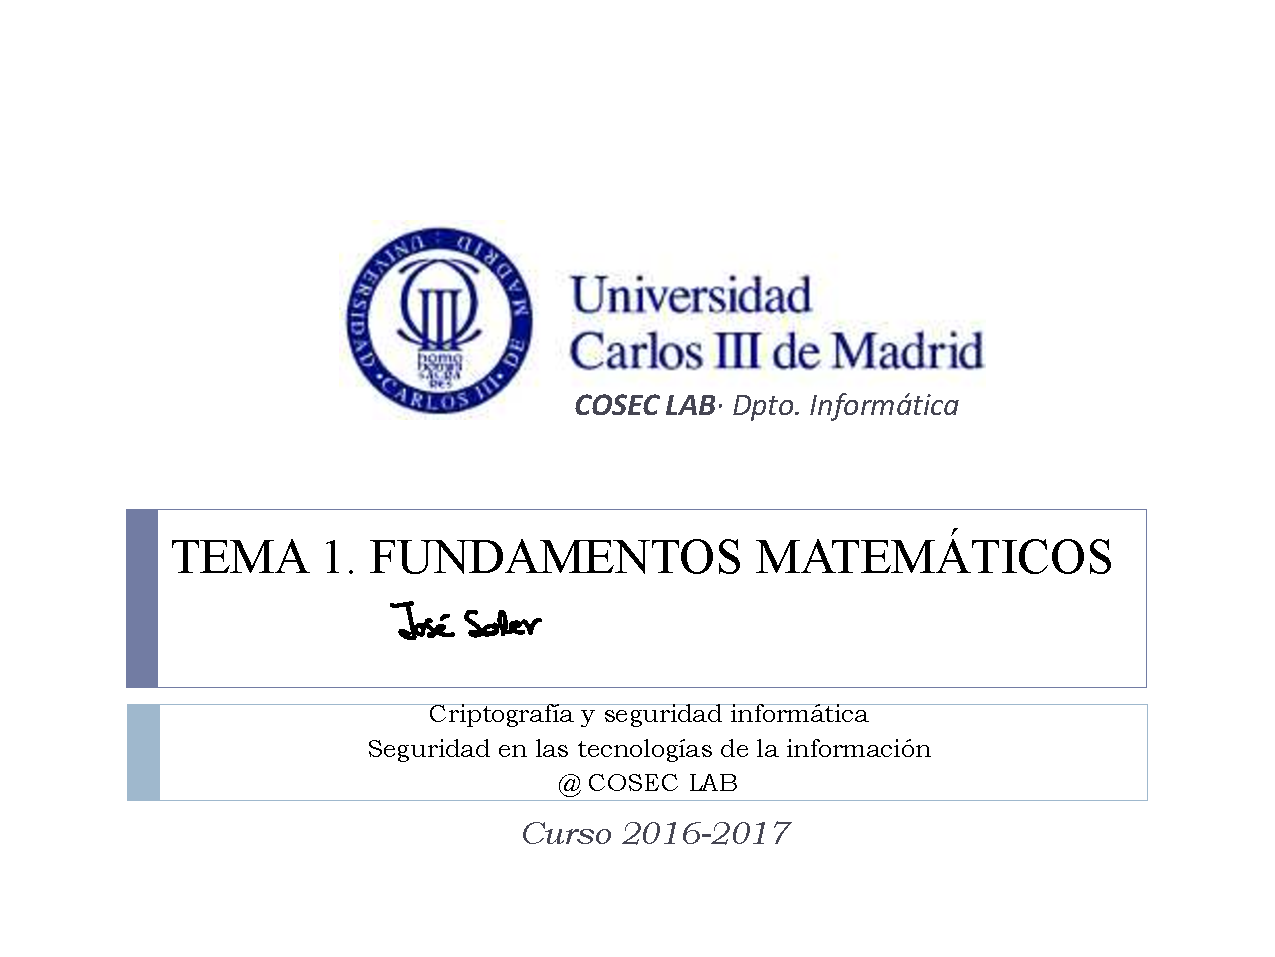
\includepdf[pages=-]{docs/Presentacion_1.2_Fundamentos_matematicos.pdf}
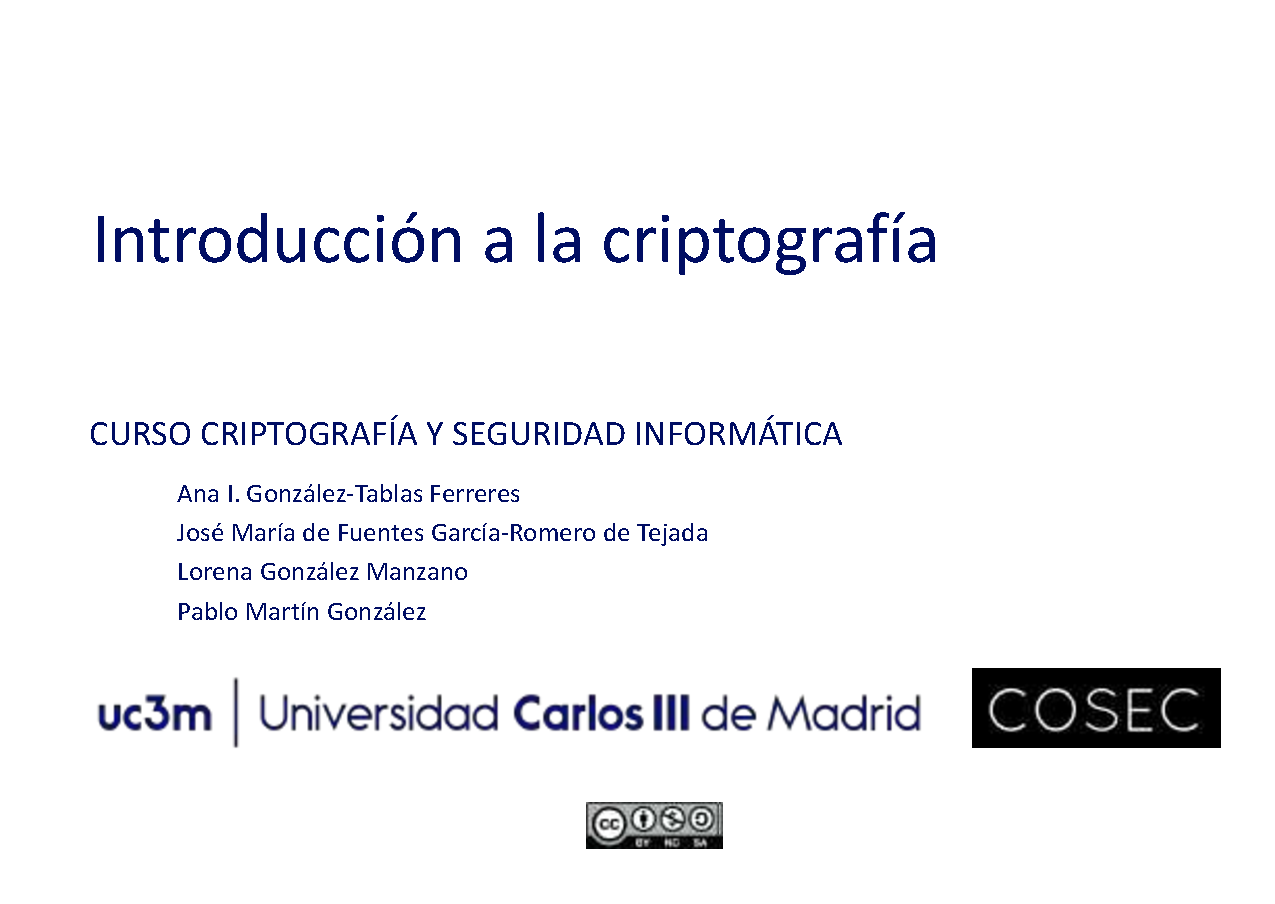
\includepdf[pages=-]{docs/Presentacion_2_(Audio).pdf}

\includepdf[pages=-]{docs/Presentacion_2.1_Introduccion_a_los_criptosistemas.pdf}

\includepdf[pages=-]{docs/Presentacion_2.2_Criptografia_clasica.pdf}

\includepdf[pages=-]{docs/Presentacion_2.3.1_Cifradores_Bloque_y_Flujo.pdf}

\includepdf[pages=-]{docs/Presentacion_2.3.2_Cifradores_Bloque_y_Flujo.pdf}
\includepdf[pages=-]{docs/Presentacion_2.3.3_Cifradores_Bloque_y_Flujo.pdf}
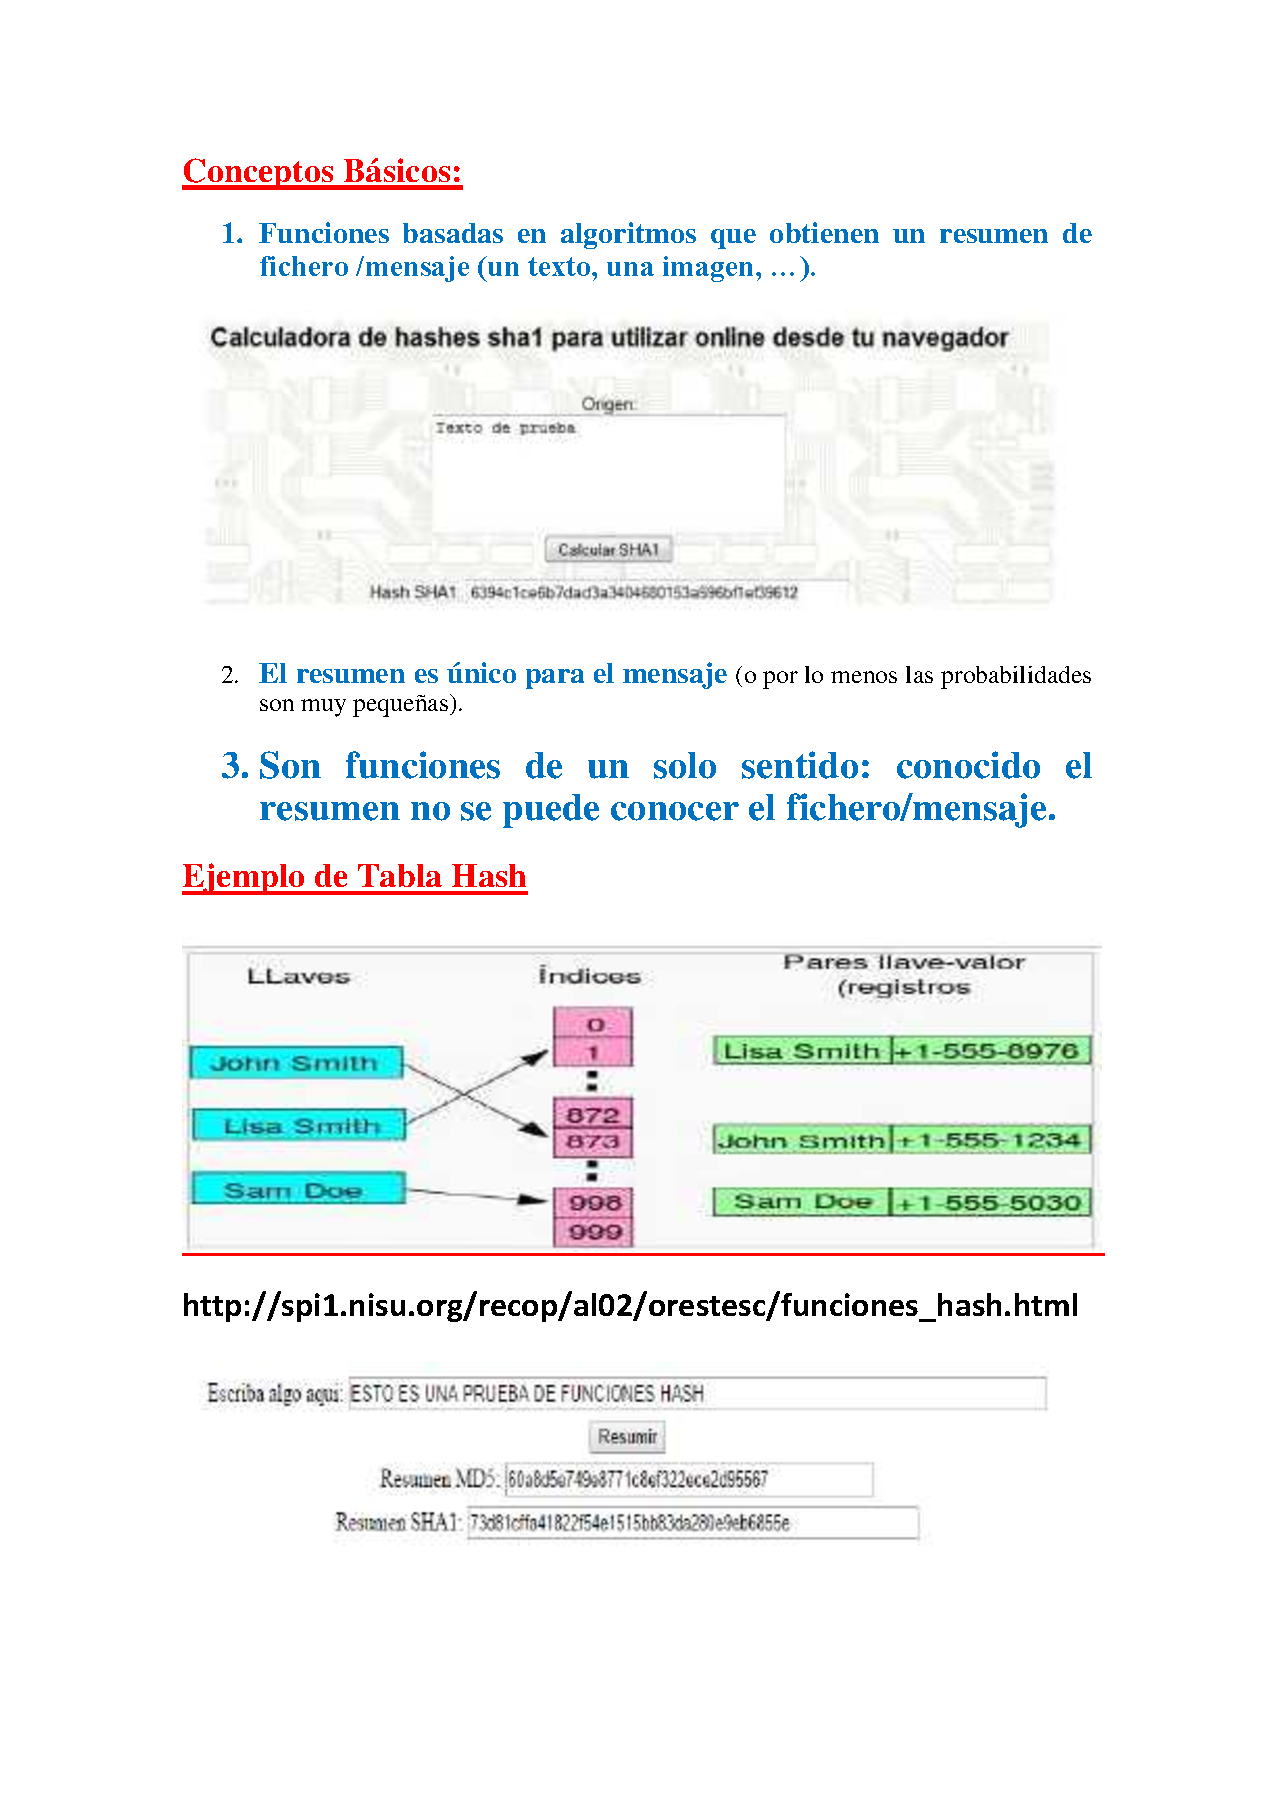
\includepdf[pages=-]{docs/Presentacion_2.4_Anexo_Resumen_Funciones_HASH.pdf}

\includepdf[pages=-]{docs/Presentacion_2.4_Funciones_Resumen_y_MAC.pdf}

\includepdf[pages=-]{docs/Presentacion_2.5.1_Cifradores_Asimetricos.pdf}
\includepdf[pages=-]{docs/Presentacion_2.5.1_Trasparencia_18.pdf}
\includepdf[pages=-]{docs/Presentacion_2.5.2_Distribucion_Claves.pdf}
\includepdf[pages=-]{docs/Presentacion_2.6_Firma_Digital.pdf}

\part{Ejercicios}
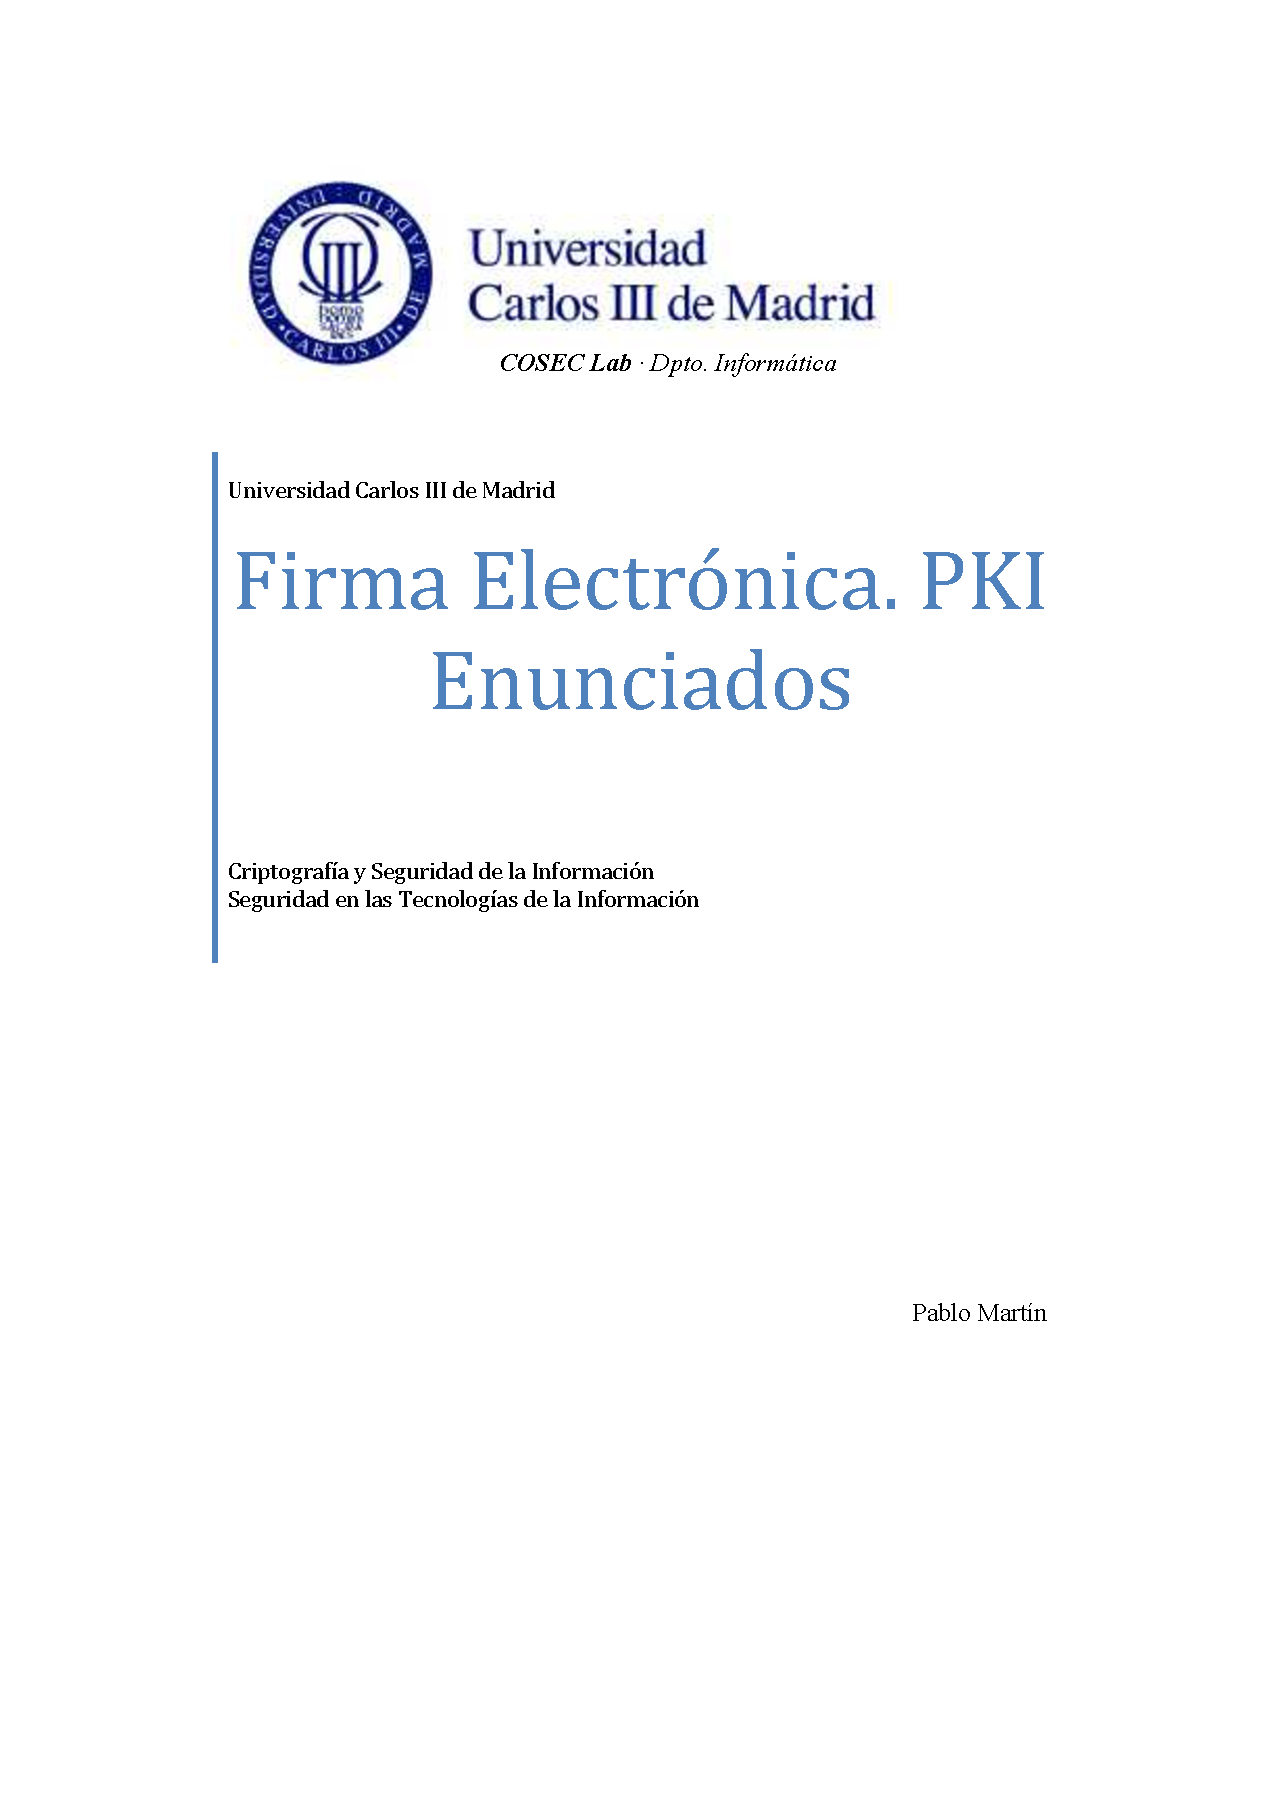
\includepdf[pages=-]{docs/CSI1617-es_Firma_Digital_y_PKI_Enunciados.pdf}
\includepdf[pages=-]{docs/Ejercicios_Examen.pdf}
\includepdf[pages=-]{docs/Enunciados_Lab_cryptool_soluciones.pdf}
\includepdf[pages=-]{docs/Enunciados_Lab_ENT_soluciones.pdf}
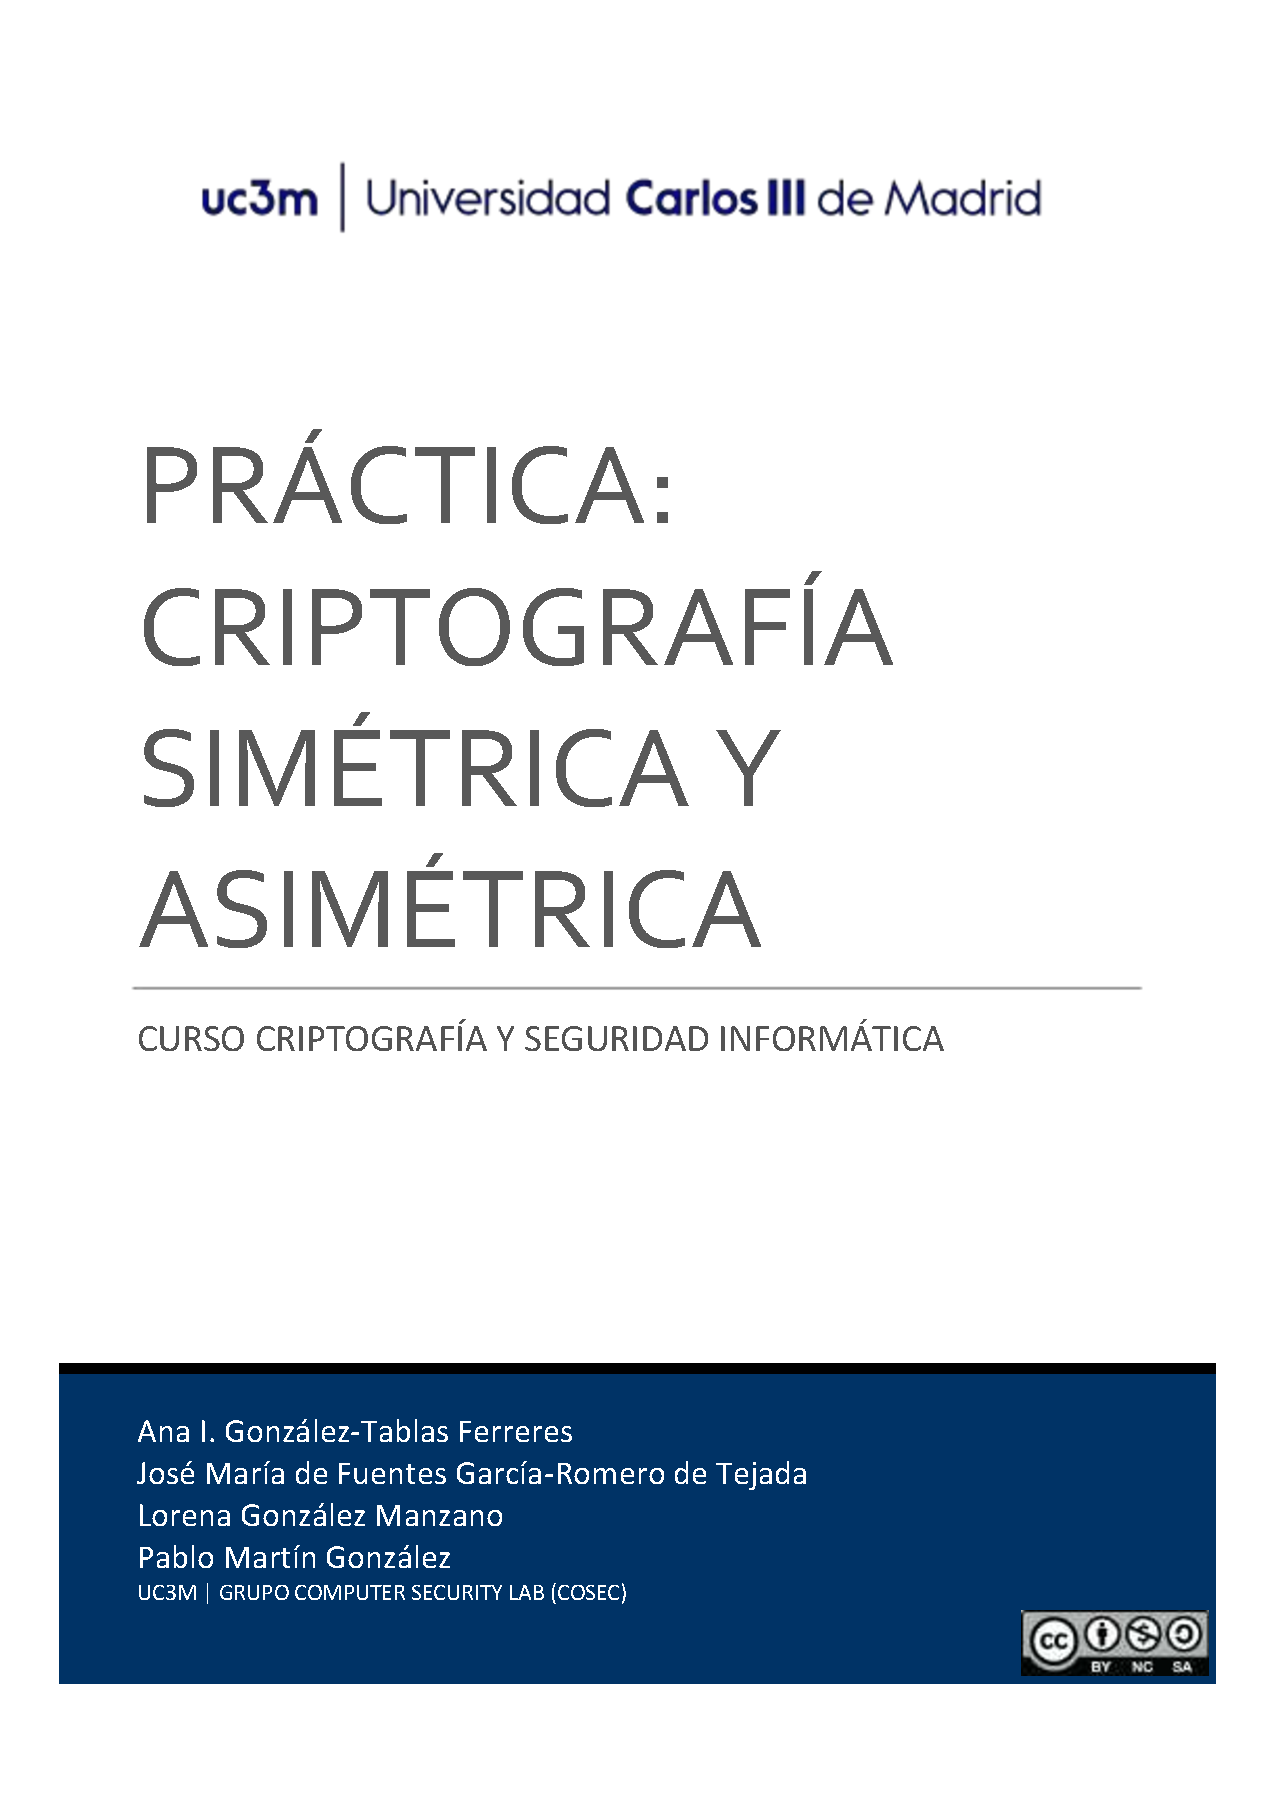
\includepdf[pages=-]{docs/Enunciados_Lab_JAVA_soluciones.pdf}
\includepdf[pages=-]{docs/Enunciados_Lab_OpenSSL_soluciones.pdf}
\includepdf[pages=-]{docs/Prob_2_ES_Enunciado.pdf}
\includepdf[pages=-]{docs/Prob_3_ES_Enunciado.pdf}
\includepdf[pages=-]{docs/Problema_PKI_adicional_ES_-_Enunciados.pdf}
\includepdf[pages=-]{docs/Problemas_1.1_Fundamentos_matematicos.pdf}
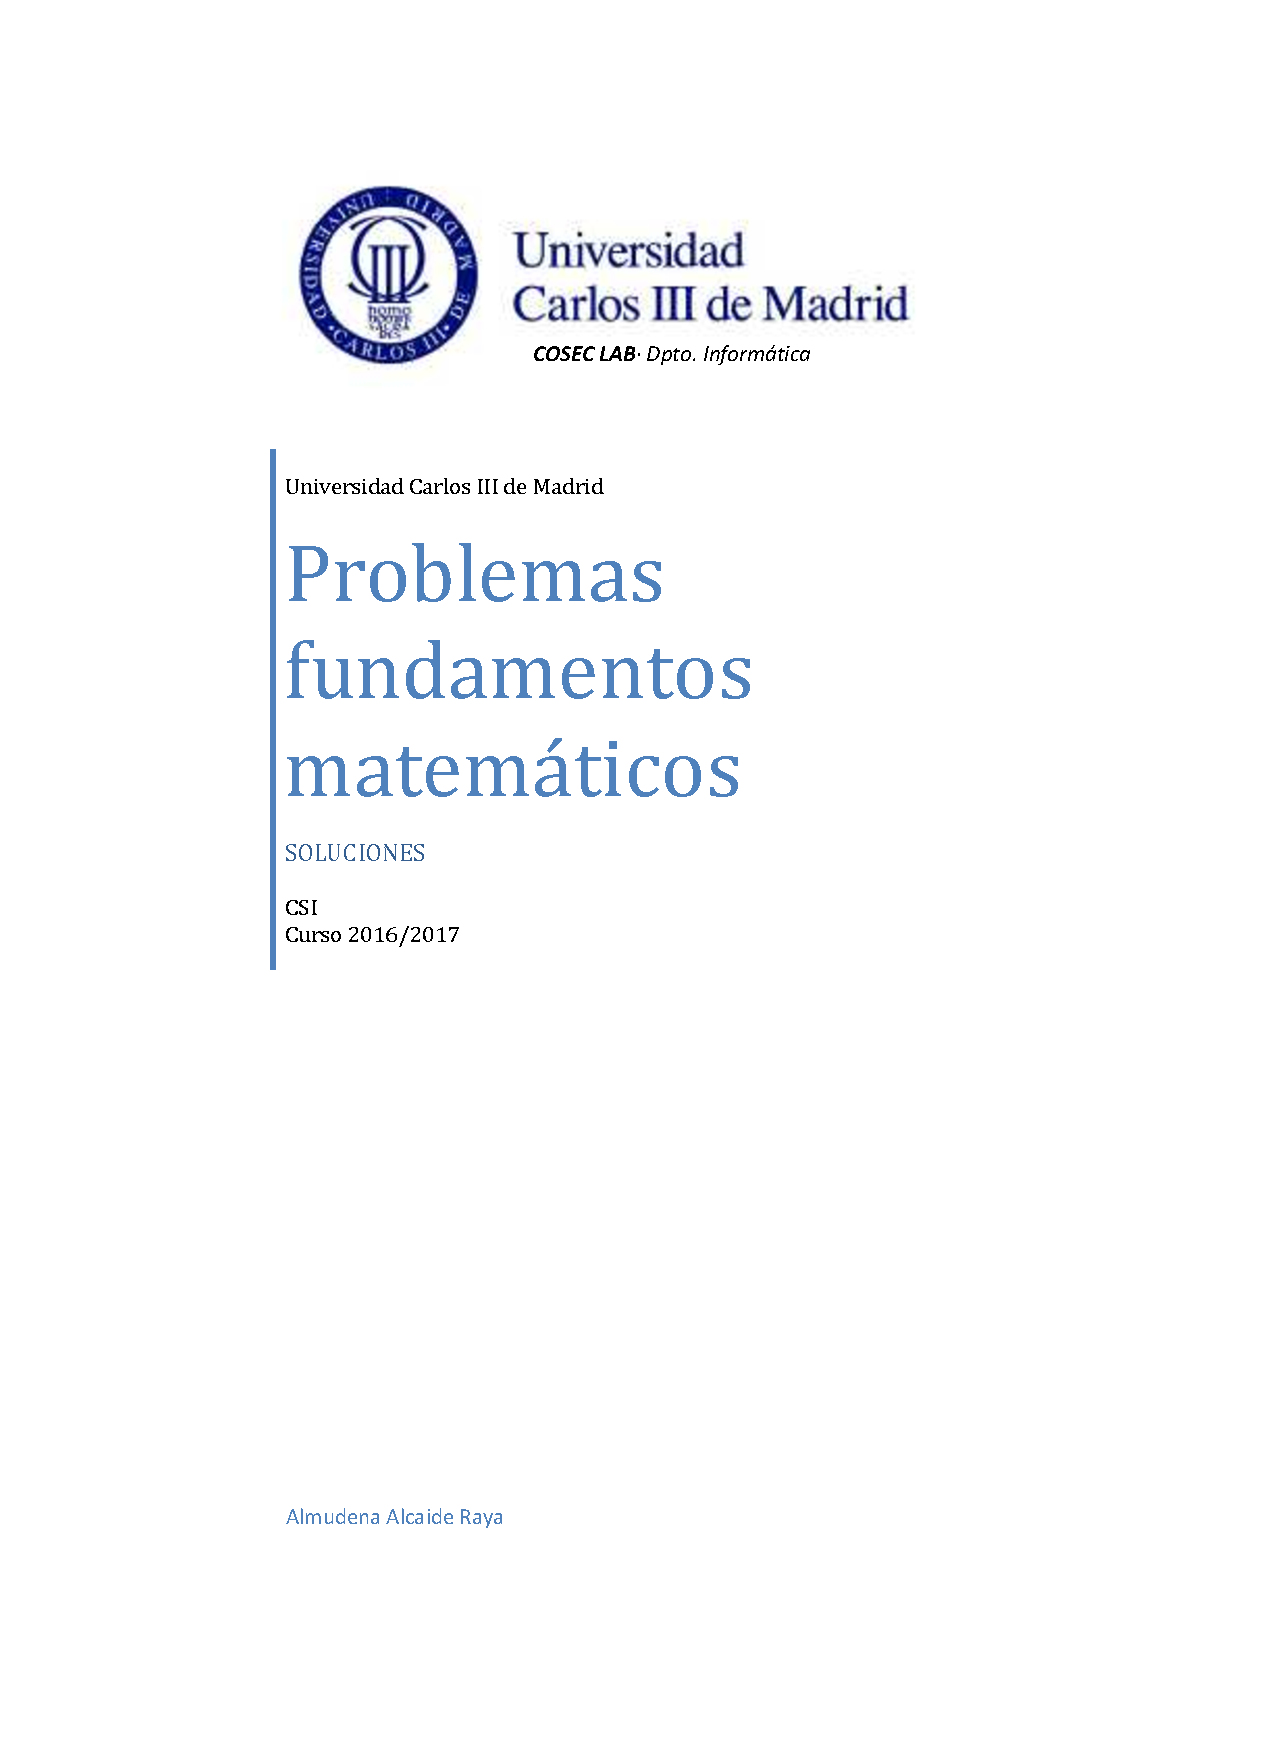
\includepdf[pages=-]{docs/Problemas_1.1_Soluciones_Fundamentos_matematicos.pdf}
\includepdf[pages=-]{docs/Problemas_1.2_Cuerpos_Galois.pdf}
\includepdf[pages=-]{docs/Problemas_1.2_Soluciones_Cuerpos_Galois.pdf}
\includepdf[pages=-]{docs/Problemas_2.2_Criptografia_clasica.pdf}
\includepdf[pages=-]{docs/Problemas_2.3_Cifrado_flujo.pdf}
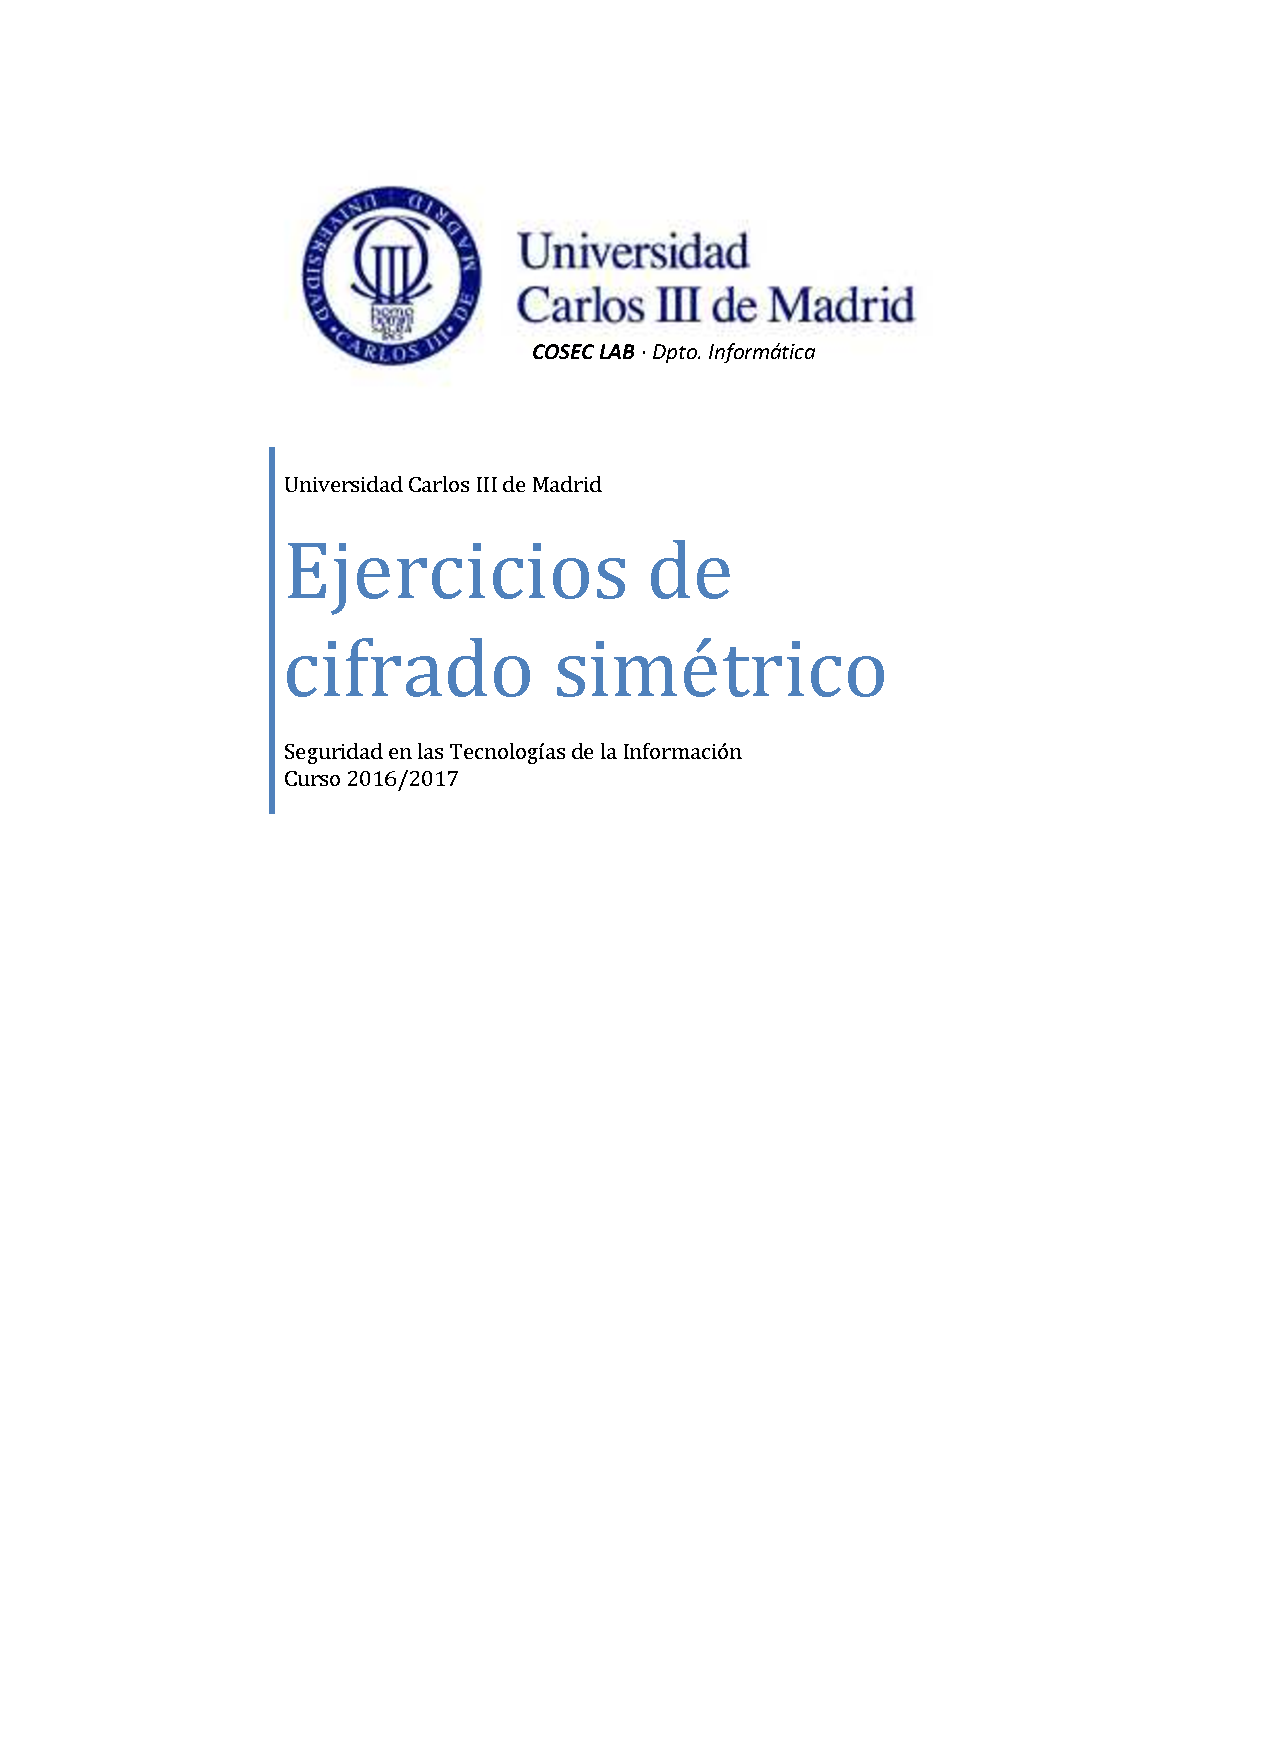
\includepdf[pages=-]{docs/Problemas_2.3_Cifrado_simetrico.pdf}
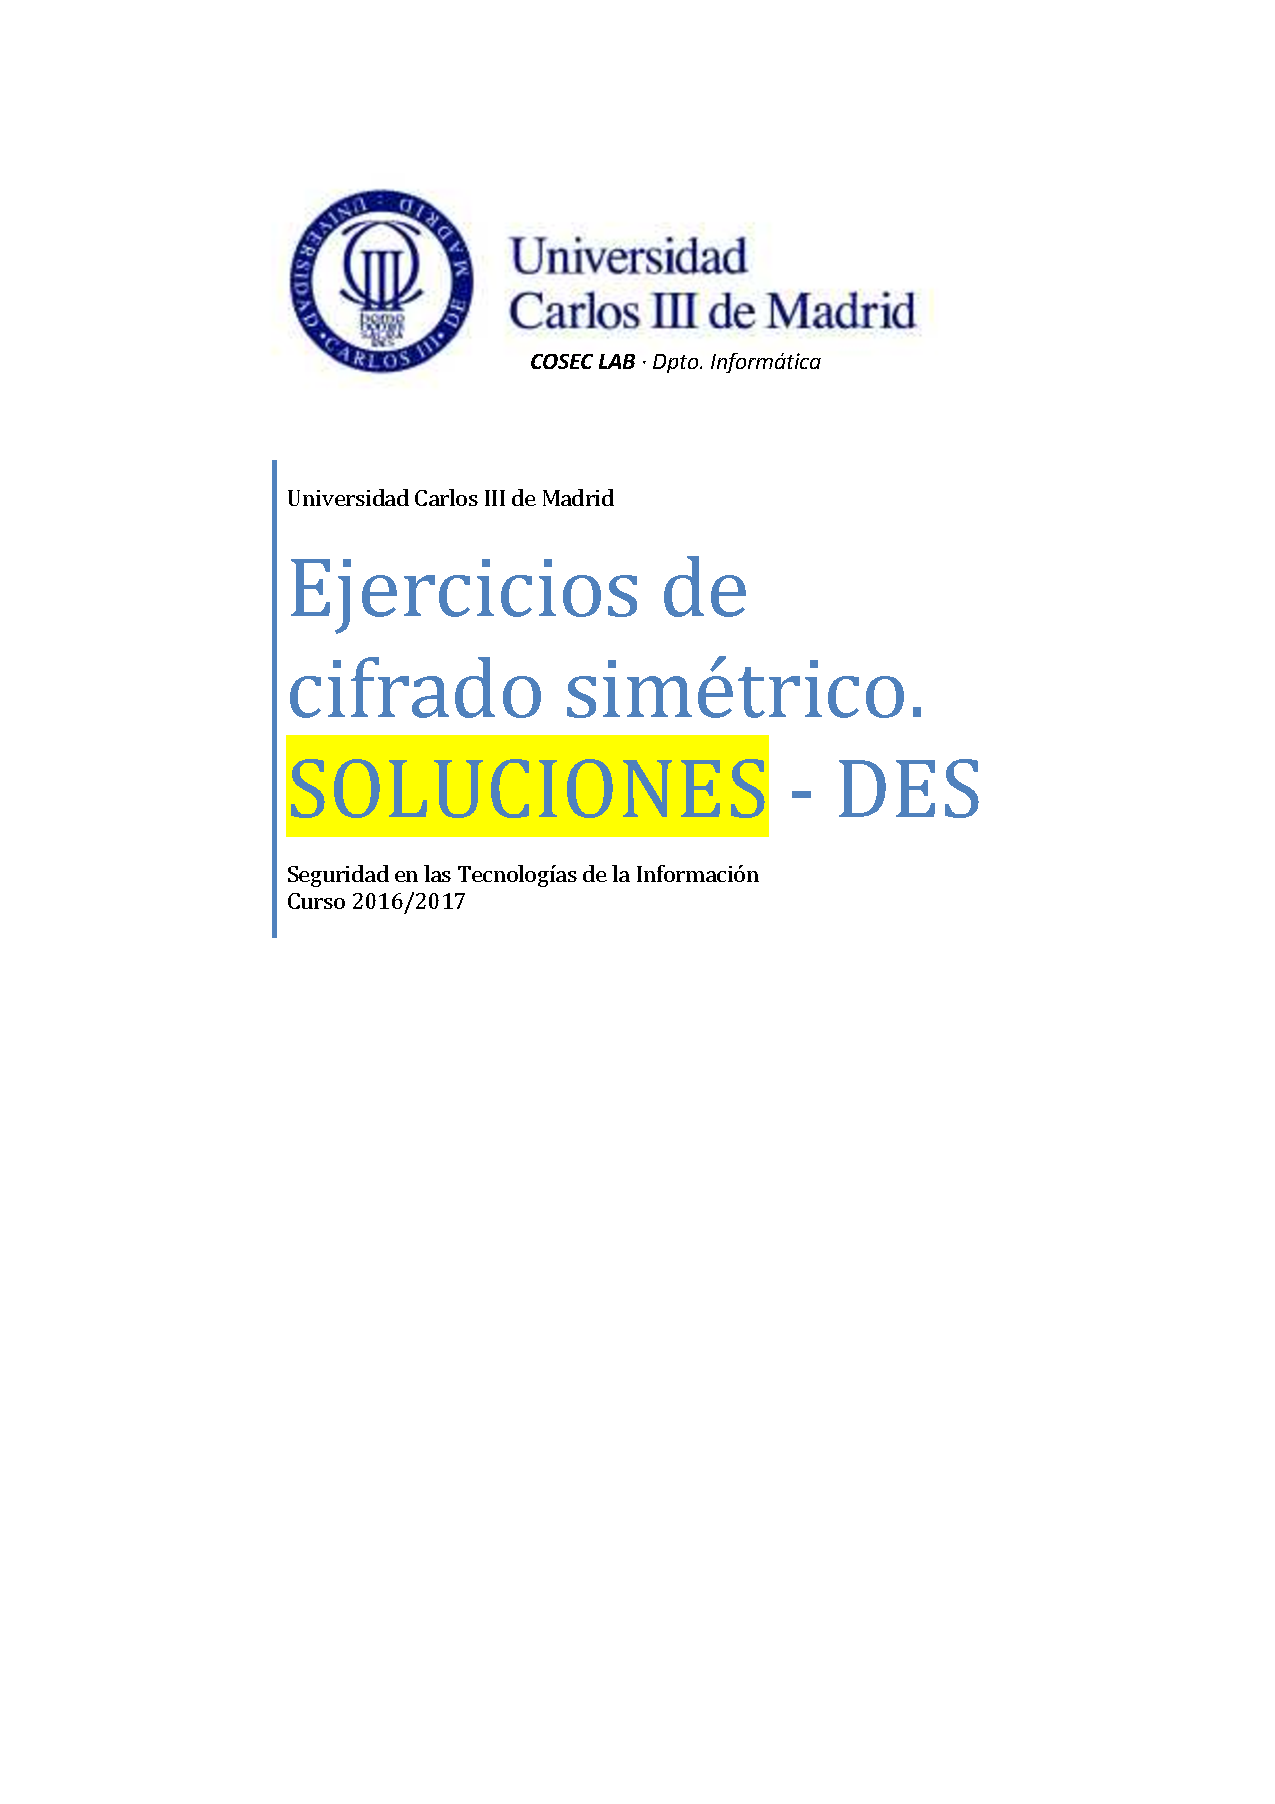
\includepdf[pages=-]{docs/Problemas_2.3.1_Soluciones_Cifrado_simetrico.pdf}
\includepdf[pages=-]{docs/Problemas_2.3.2_Soluciones_Cifrado_simetrico.pdf}
\includepdf[pages=-]{docs/Problemas_2.5_Cifrado_Asimetrico.pdf}
\includepdf[pages=-]{docs/Problemas_2.5_Distribucion_Claves.pdf}
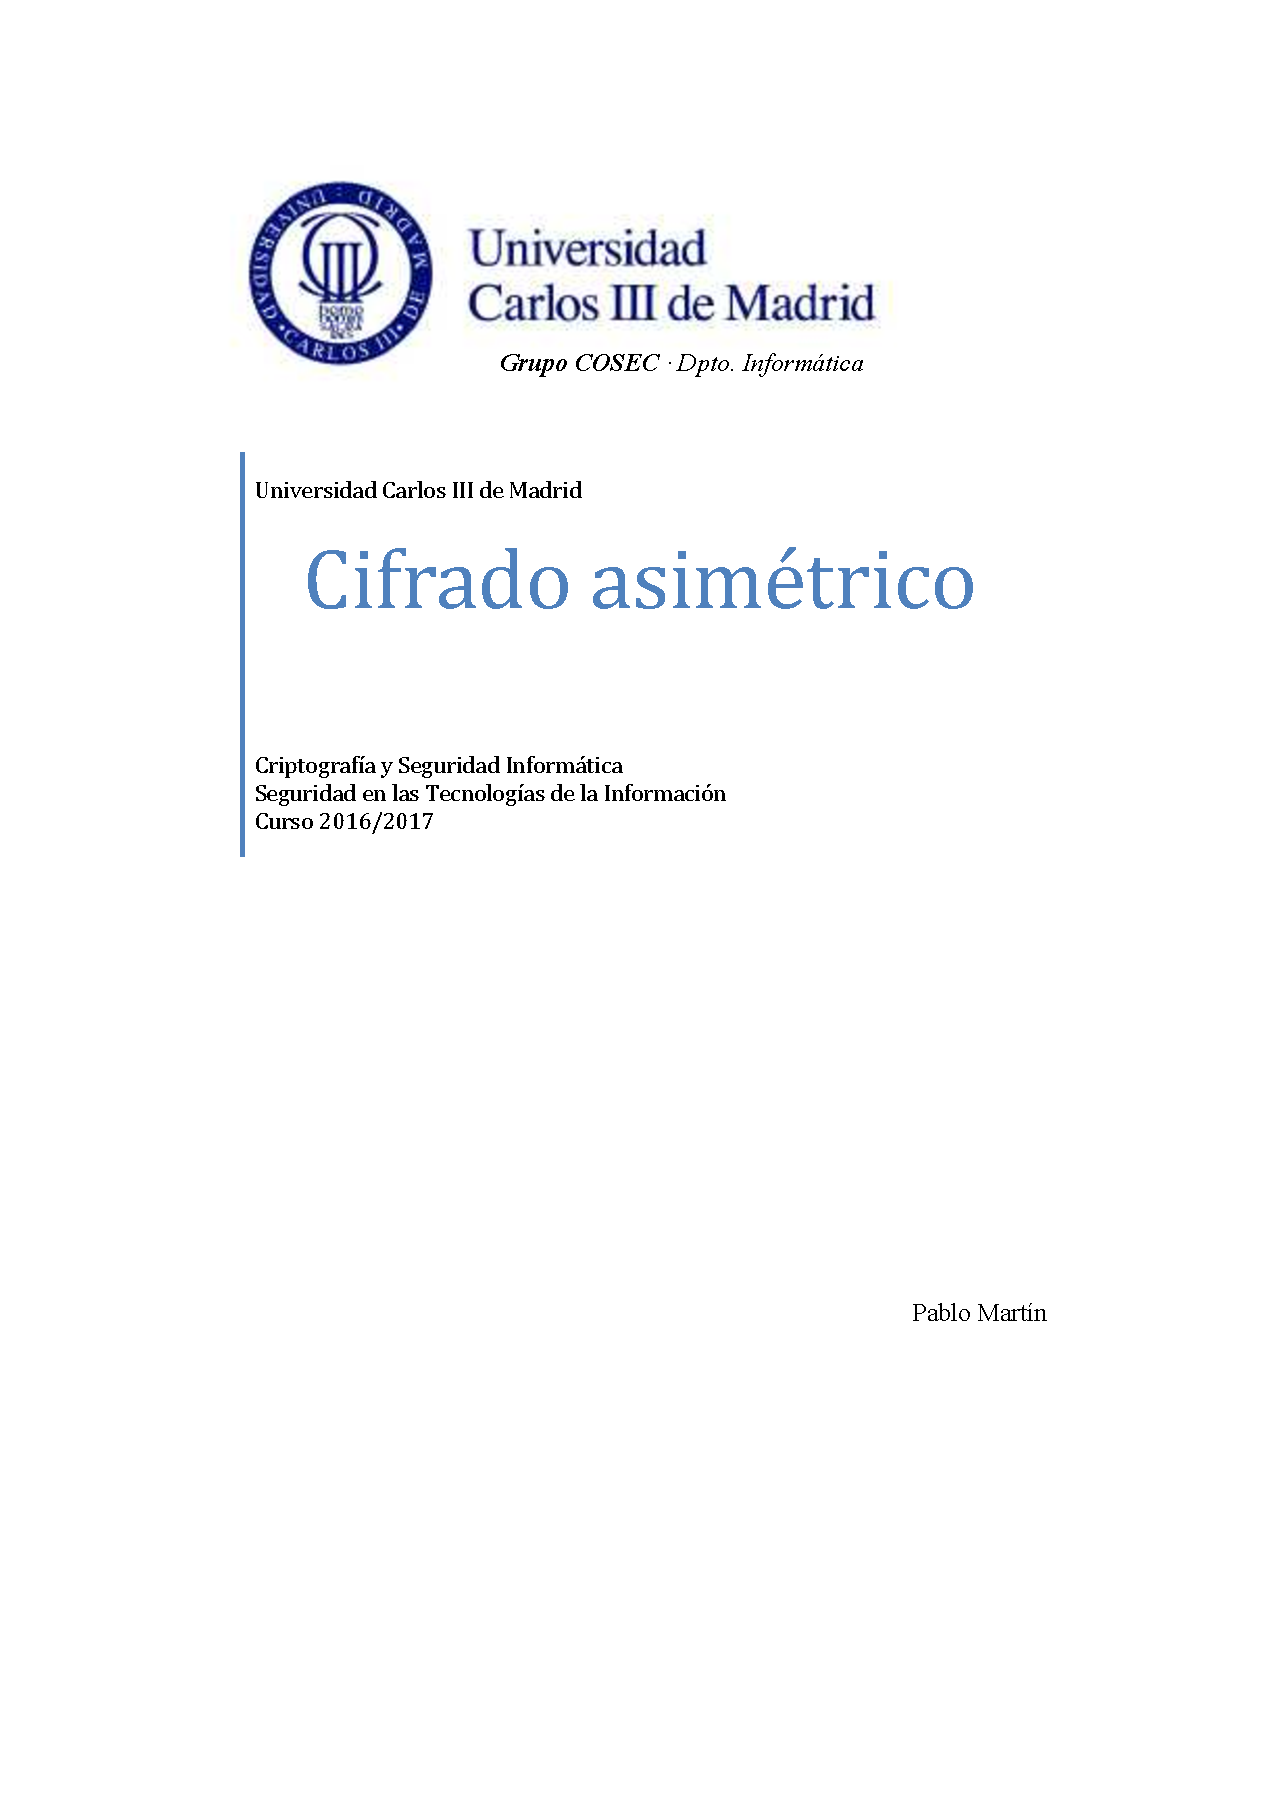
\includepdf[pages=-]{docs/Problemas_2.5_Soluciones_Cifrado_Asimetrico.pdf}
\includepdf[pages=-]{docs/Problemas_2.5_Soluciones_Distribucion_Claves.pdf}
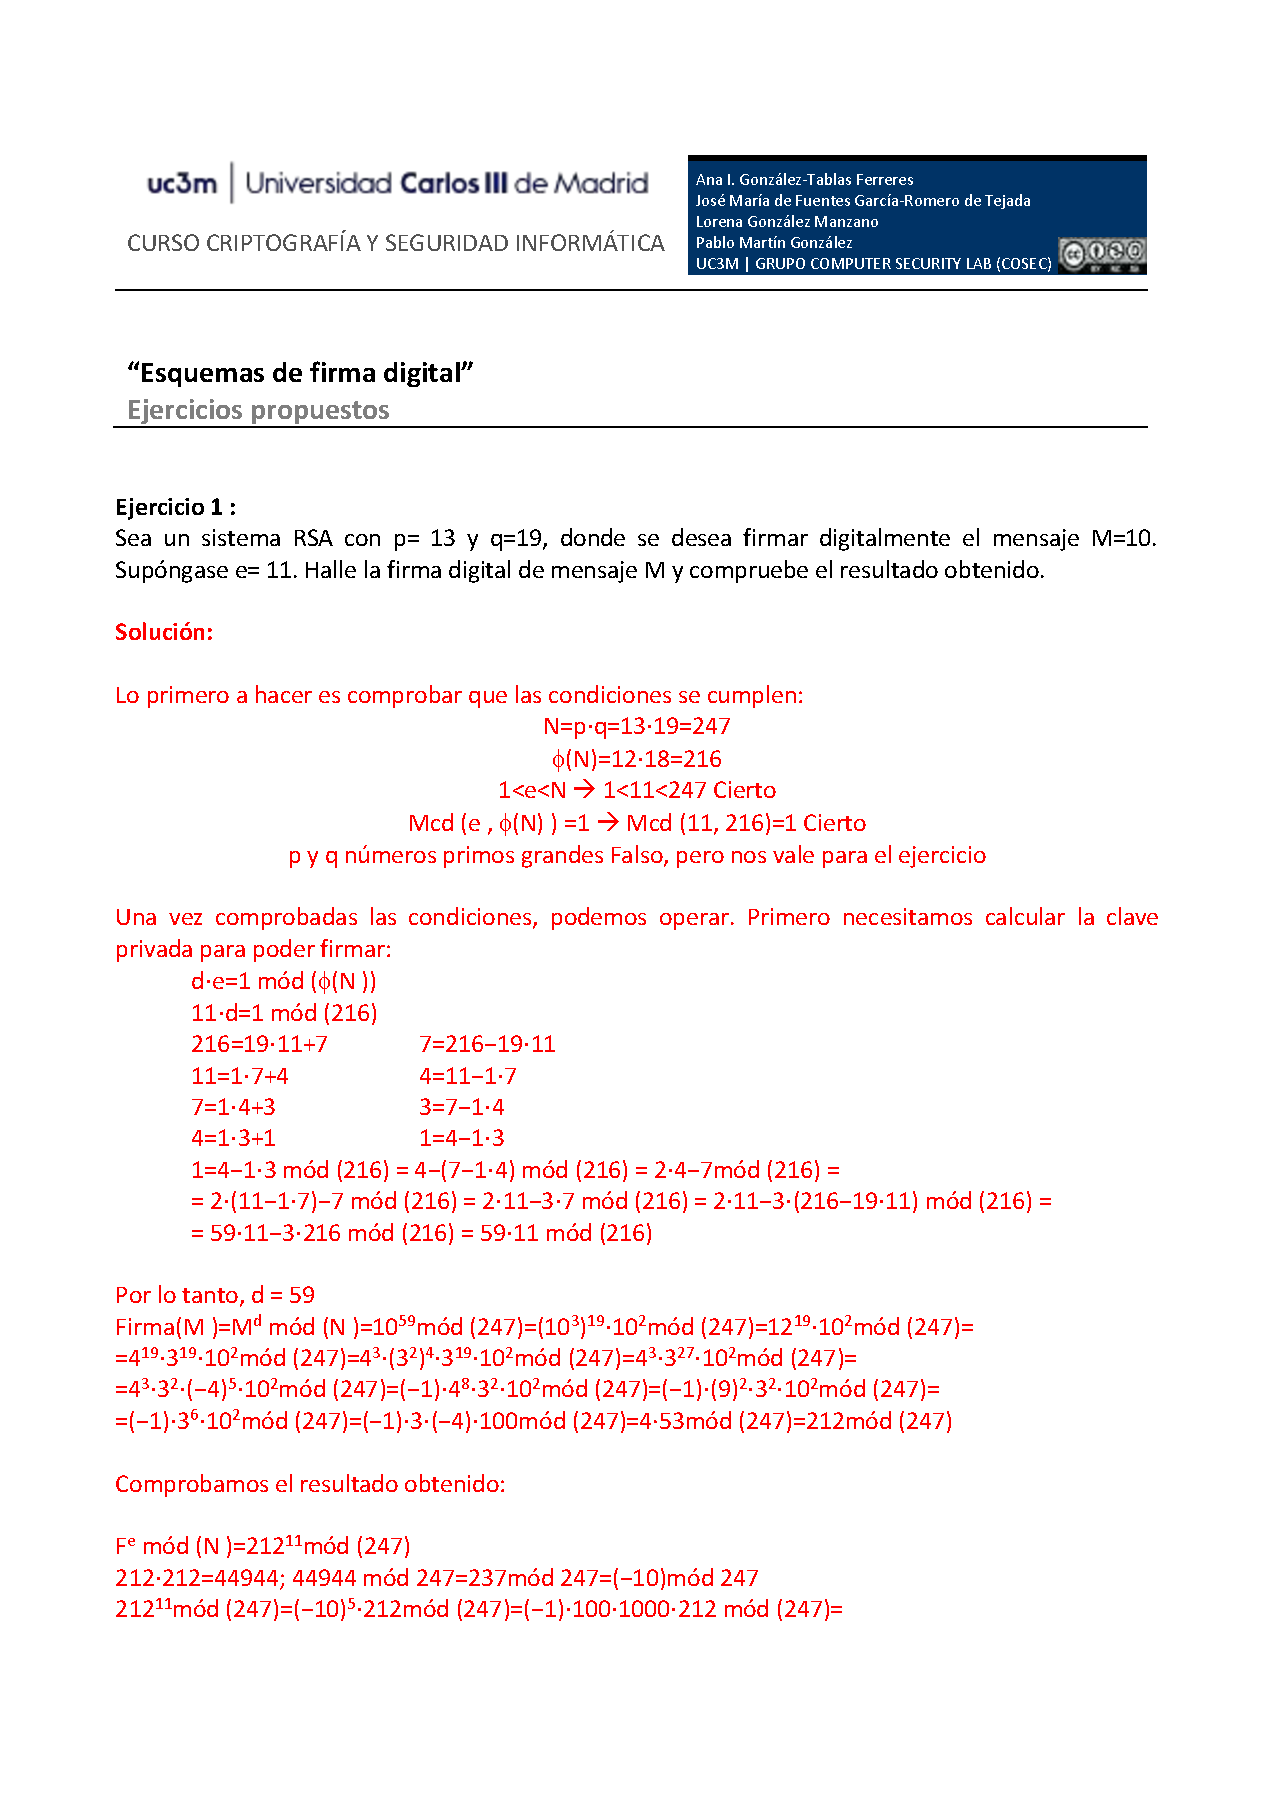
\includepdf[pages=-]{docs/Problemas_2.7_Firma_Digital_Soluciones.pdf}
\includepdf[pages=-]{docs/Problemas_2.7_Firma_Digital_y_PKI.pdf}
\includepdf[pages=-]{docs/Problemas_2.7_PKI_Soluciones.pdf}

\part{ractica final}
\includepdf[pages=-]{docs/EXAMEN_ES.pdf}
\includepdf[pages=-]{docs/MemoriaCSI.Grupo16.pdf}

\part{Exámenes}
\includepdf[pages=-]{docs/ExamenCSI.pdf}
\includepdf[pages=-]{docs/TEST_L13_autenti_sol.pdf}
\includepdf[pages=-]{docs/TEST_L12_InfraestructurasClavePublica_soluciones.pdf}
\includepdf[pages=-]{docs/TEST_L11_EsquemasFirmaDigital_soluciones.pdf}
\includepdf[pages=-]{docs/TEST_L10_MAC_sol.pdf}
\includepdf[pages=-]{docs/TEST_L8_DistribucionEstablecimientoClave_soluciones.pdf}
\includepdf[pages=-]{docs/TEST_L6_cifrado_flujo_sol.pdf}
\includepdf[pages=-]{docs/TEST_L5_cifrado_simetrico_sol.pdf}
\includepdf[pages=-]{docs/TEST_L4_criptoClasica_sol.pdf}
\includepdf[pages=-]{docs/TEST_L2_L3-IntroCripto_y_ConceptoRela-FundamenMate_sol.pdf}
\includepdf[pages=-]{docs/TEST_L1-FundamenMate_sol.pdf}
\includepdf[pages=-]{docs/TEST__L9_fun_resum_sol.pdf}
\includepdf[pages=-]{docs/ExamenFinalMayo2014conPortada.pdf}
\includepdf[pages=-]{docs/ExamenFinalMayo2013conPortada.pdf}
\includepdf[pages=-]{docs/TEST_L7_CriptosistemasAsimetricos_soluciones.pdf}
\includepdf[pages=-]{docs/Prob_3_ES_Enunciado.pdf}
\includepdf[pages=-]{docs/Prob_2_ES_Enunciado.pdf}
\includepdf[pages=-]{docs/Prob_1_ES_Enunciado.pdf}
\includepdf[pages=-]{docs/Ejercicios_L12_Infraestructuras_Clave_Publica_Soluciones.pdf}
\includepdf[pages=-]{docs/Ejercicios_L11_Esquemas_firma_digital_Soluciones.pdf}
\includepdf[pages=-]{docs/Ejercicios_L8_Distribucion_establecimiento_clave_Soluciones.pdf}
\includepdf[pages=-]{docs/Ejercicios_L7_Criptosistemas_asimetricos_Soluciones.pdf}
\includepdf[pages=-]{docs/Ejercicios_L6_sol.pdf}
\includepdf[pages=-]{docs/Ejercicios_L5_Soluciones.pdf}
\includepdf[pages=-]{docs/Ejercicios_L4_sol.pdf}
\includepdf[pages=-]{docs/Ejercicios_L1_sol.pdf}
\includepdf[pages=-]{docs/EjercicioAdicionalExamenEnunciado.pdf}

\part{Lab 1}
\includepdf[pages=-]{docs/CrypToolENT.pdf}
\includepdf[pages=-]{docs/Enunciados_Lab_cryptool_1920.pdf}
\includepdf[pages=-]{docs/Enunciados_Lab_ENT_1920.pdf}

\part{Lab 2}
\includepdf[pages=-]{docs/BouncyCastle.pdf}
\includepdf[pages=-]{docs/LAB2_Enunciado-19_20.pdf}

\part{Lab 3}
\includepdf[pages=-]{docs/OpenSSL.pdf}
\includepdf[pages=-]{docs/CSI1920-es_OpenSSL_-_enunciados.pdf}

\part{Practicas}
\includepdf[pages=-]{docs/Enunciados_Lab_cryptool_soluciones.pdf}
\includepdf[pages=-]{docs/Enunciados_Lab_cryptool.pdf}
\includepdf[pages=-]{docs/Enunciados_Lab_ENT_soluciones.pdf}
\includepdf[pages=-]{docs/Enunciados_Lab_ENT.pdf}
\includepdf[pages=-]{docs/Enunciados_Lab_JAVA_soluciones.pdf}
\includepdf[pages=-]{docs/Enunciados_Lab_JAVA.pdf}
\includepdf[pages=-]{docs/Enunciados_Lab_OpenSSL_soluciones.pdf}
\includepdf[pages=-]{docs/Enunciados_Lab_OpenSSL.pdf}

\part{Recursos}
\includepdf[pages=-]{docs/Stallings_Cryptography_and_Network_Security.pdf}

\end{document}